\section{Introduction}

For this report we evaluate the capabilities of texture-features extracted with the Leung-Malik (LM) filter bank of finding images similar to a given one. In the following sections we will extract descriptors based on texture filters and then use a knn-search algorithm to retrieve the most fitting images.

\section{Leung-Malik Filter Bank}

We use the Matlab code provided by the Visual Geometry Group of Oxford University to create the LM filter bank\footnote{\url{http://www.robots.ox.ac.uk/\~vgg/research/texclass/filters.html}}. The bank consists of 48 different filters at different scales and orientations: 36 first and second derivatives of Gaussians at 6 different orientations and 3 scales, 8 Laplacian of Gaussian (LOG) filters, and 4 Gaussian filters. Figure \ref{fig:lmFilter} shows the filters visualized as heat maps.

\begin{figure}[!hbt]
  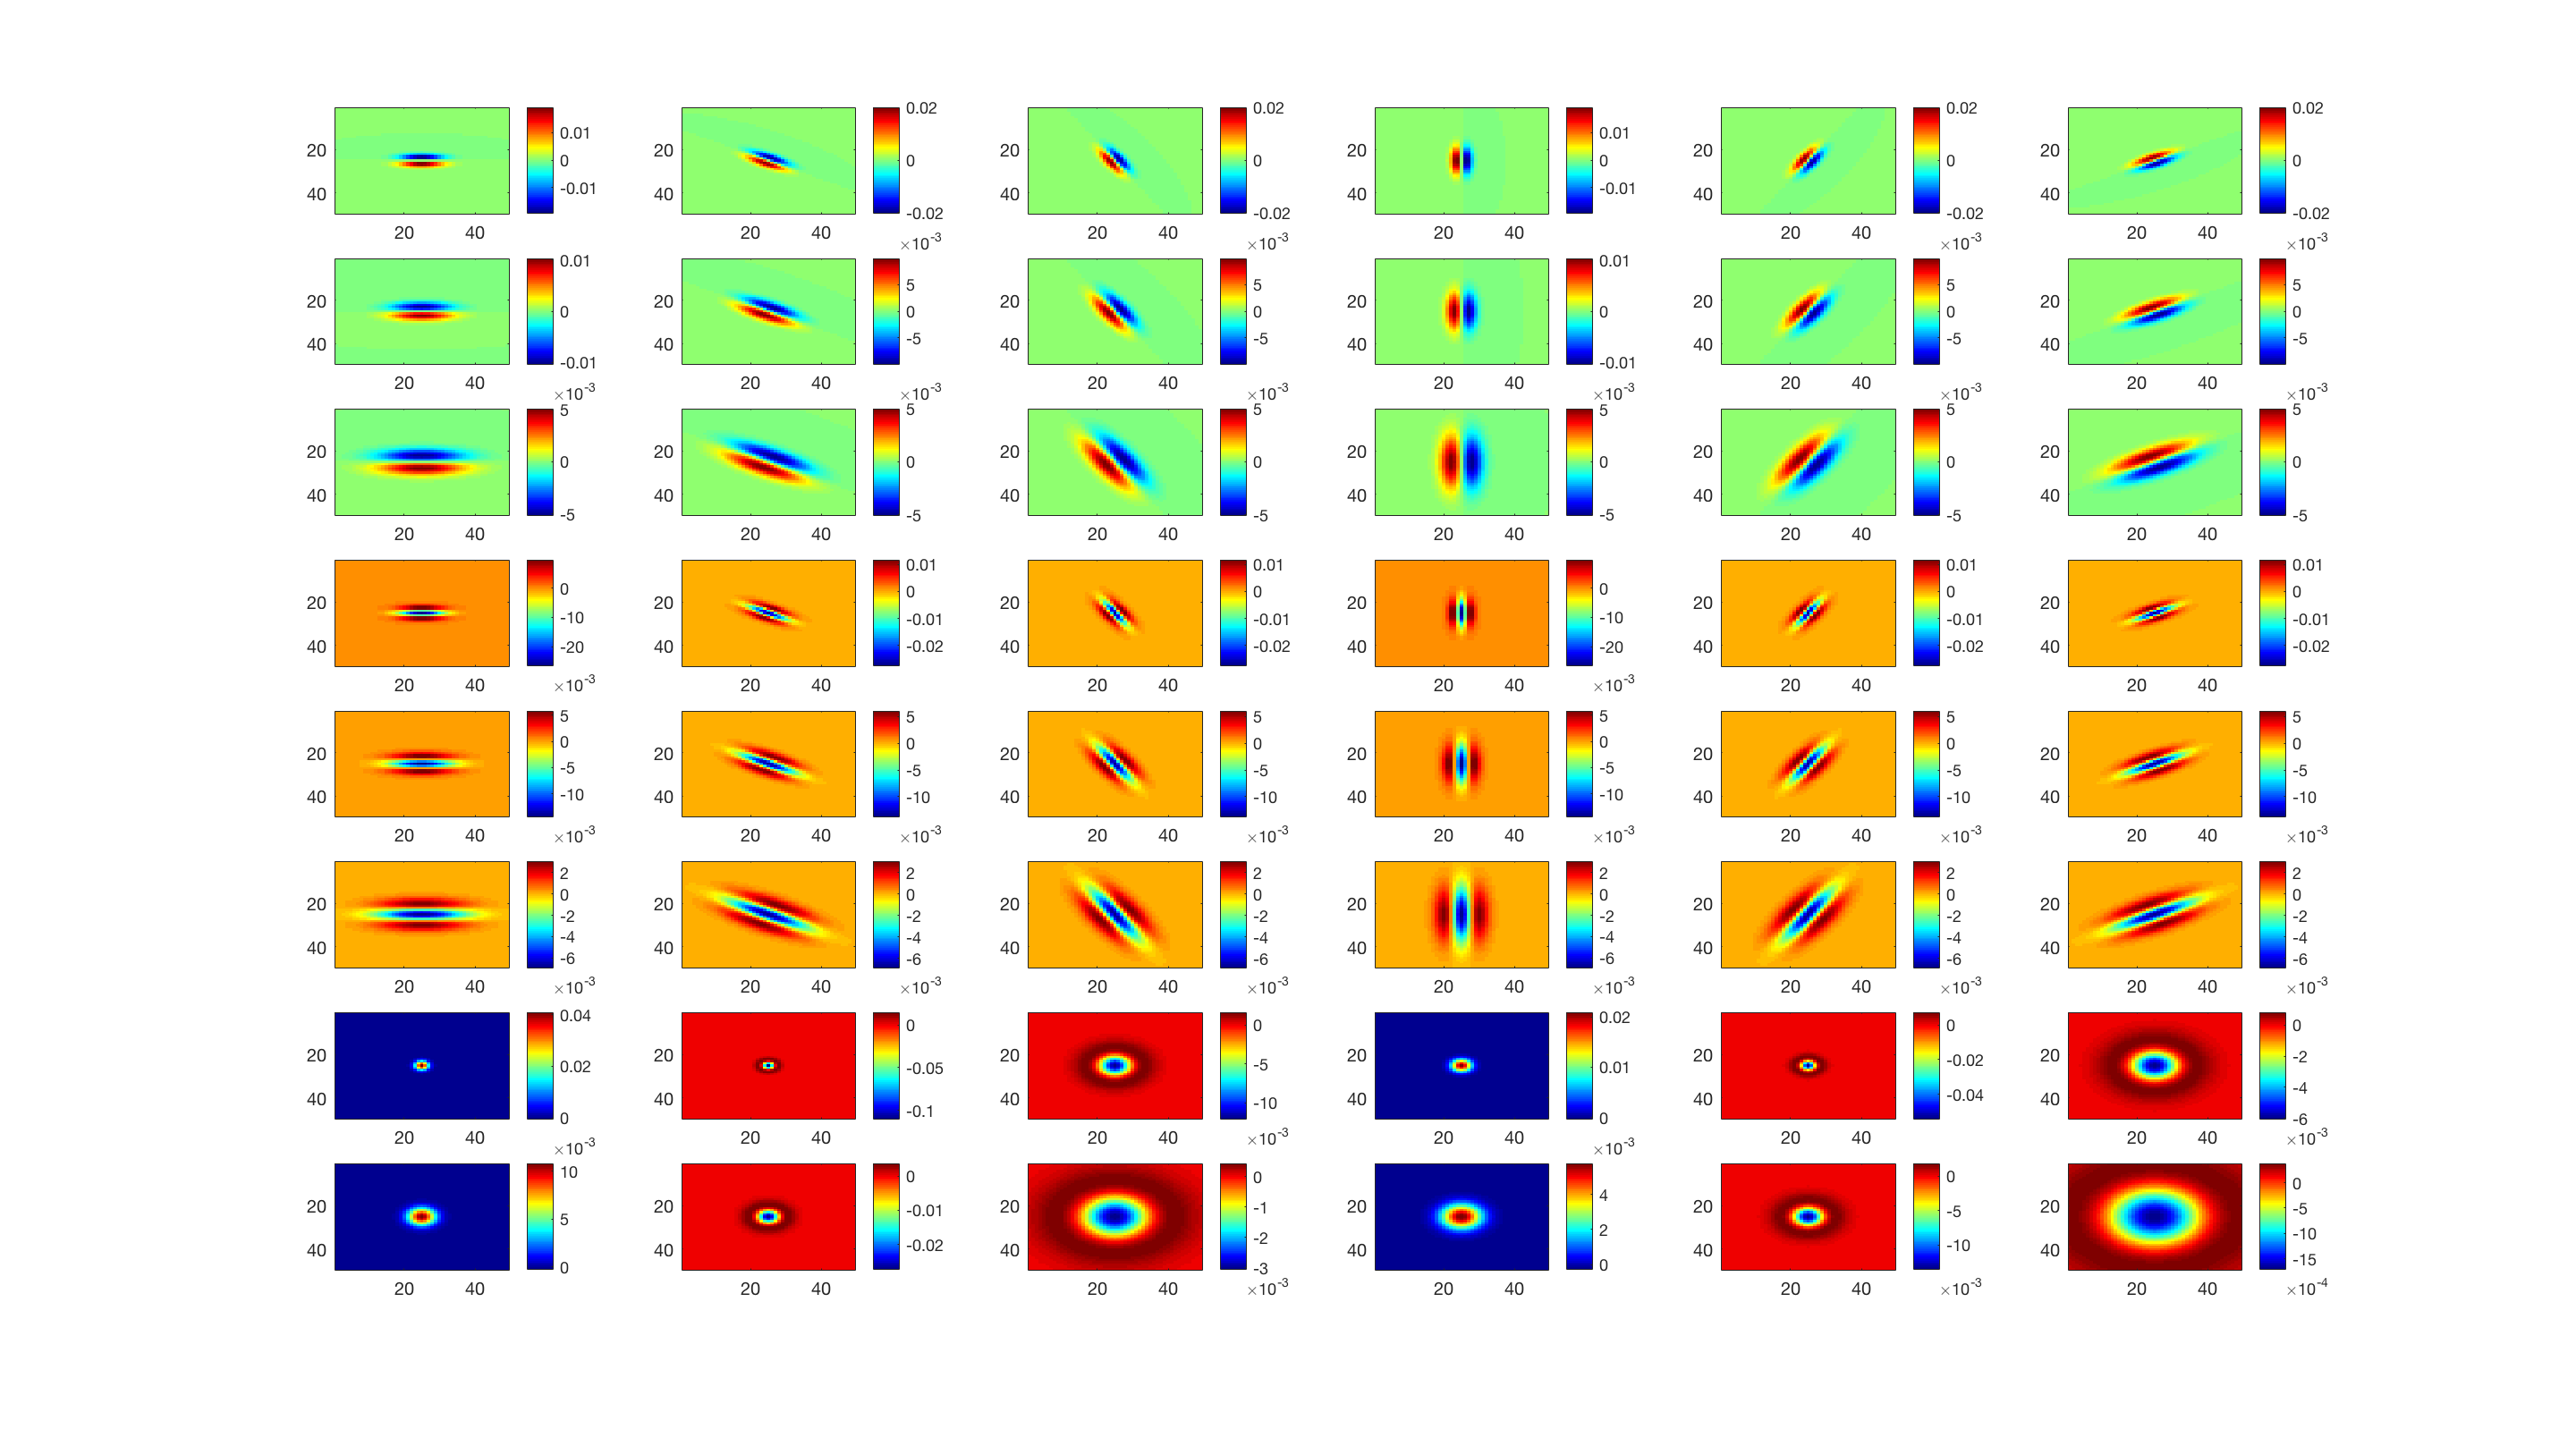
\includegraphics[width=\textwidth]{img/LM_filter_bank}
  \caption{Visualization of LM filter bank}
  \label{fig:lmFilter}
\end{figure}


\section{Texture Descriptors}

To obtain expressive descriptors that describe the texture of an image, we use the responses of the image to the convolutional filters of the LM filter bank. 

\begin{figure}[!hbt]
  \centering
  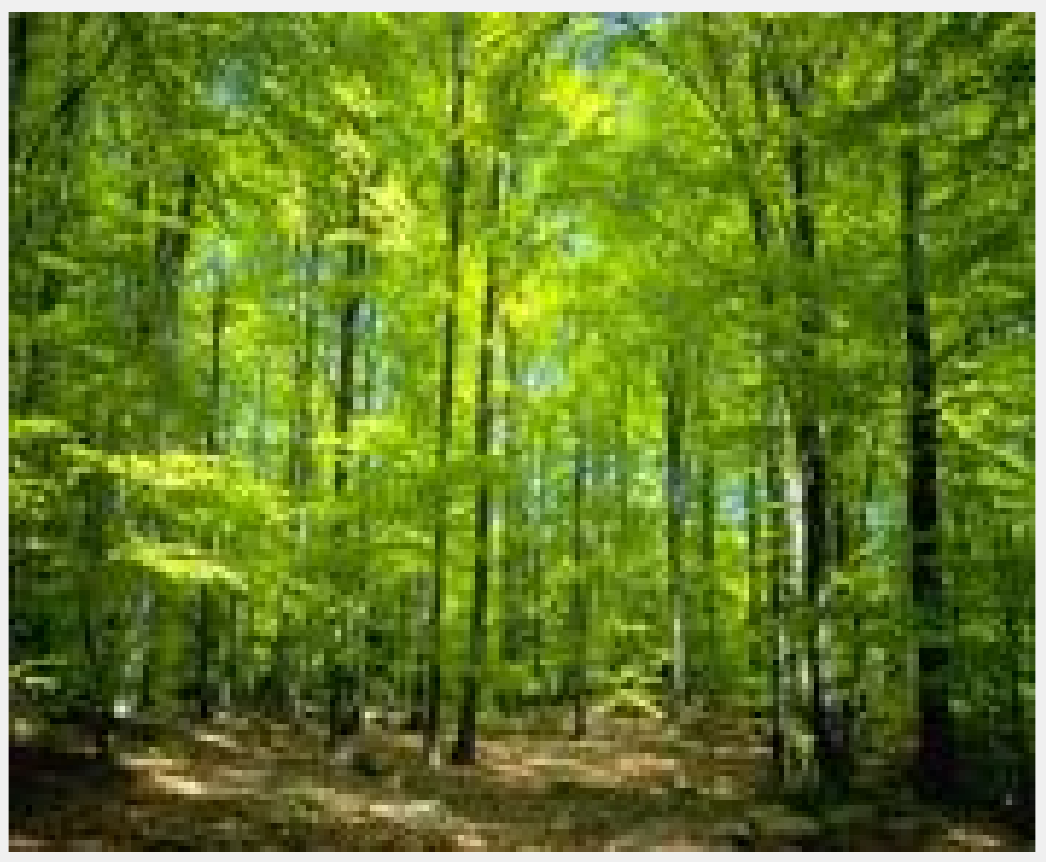
\includegraphics[width=0.4\textwidth]{img/f9}
  \caption{Example image \texttt{forest\_9}}
  \label{fig:f9ResponseA}
\end{figure}

Figure \ref{fig:f9ResponseB} shows the response of the image \texttt{forest\_9} on all 48 filters (to compare filters and responses, also see figure \ref{fig:lmFilter}). In figure \ref{fig:f9ResponseA} we show the original image in RGB colors. Figure \ref{fig:f9ResponseB} depicts the responses of the same image after being converted to grayscale to all 48 filters as a heatmap with blue corresponding to low responses and red corresponding to high responses.

\begin{figure}[!hbt]
  \centering
  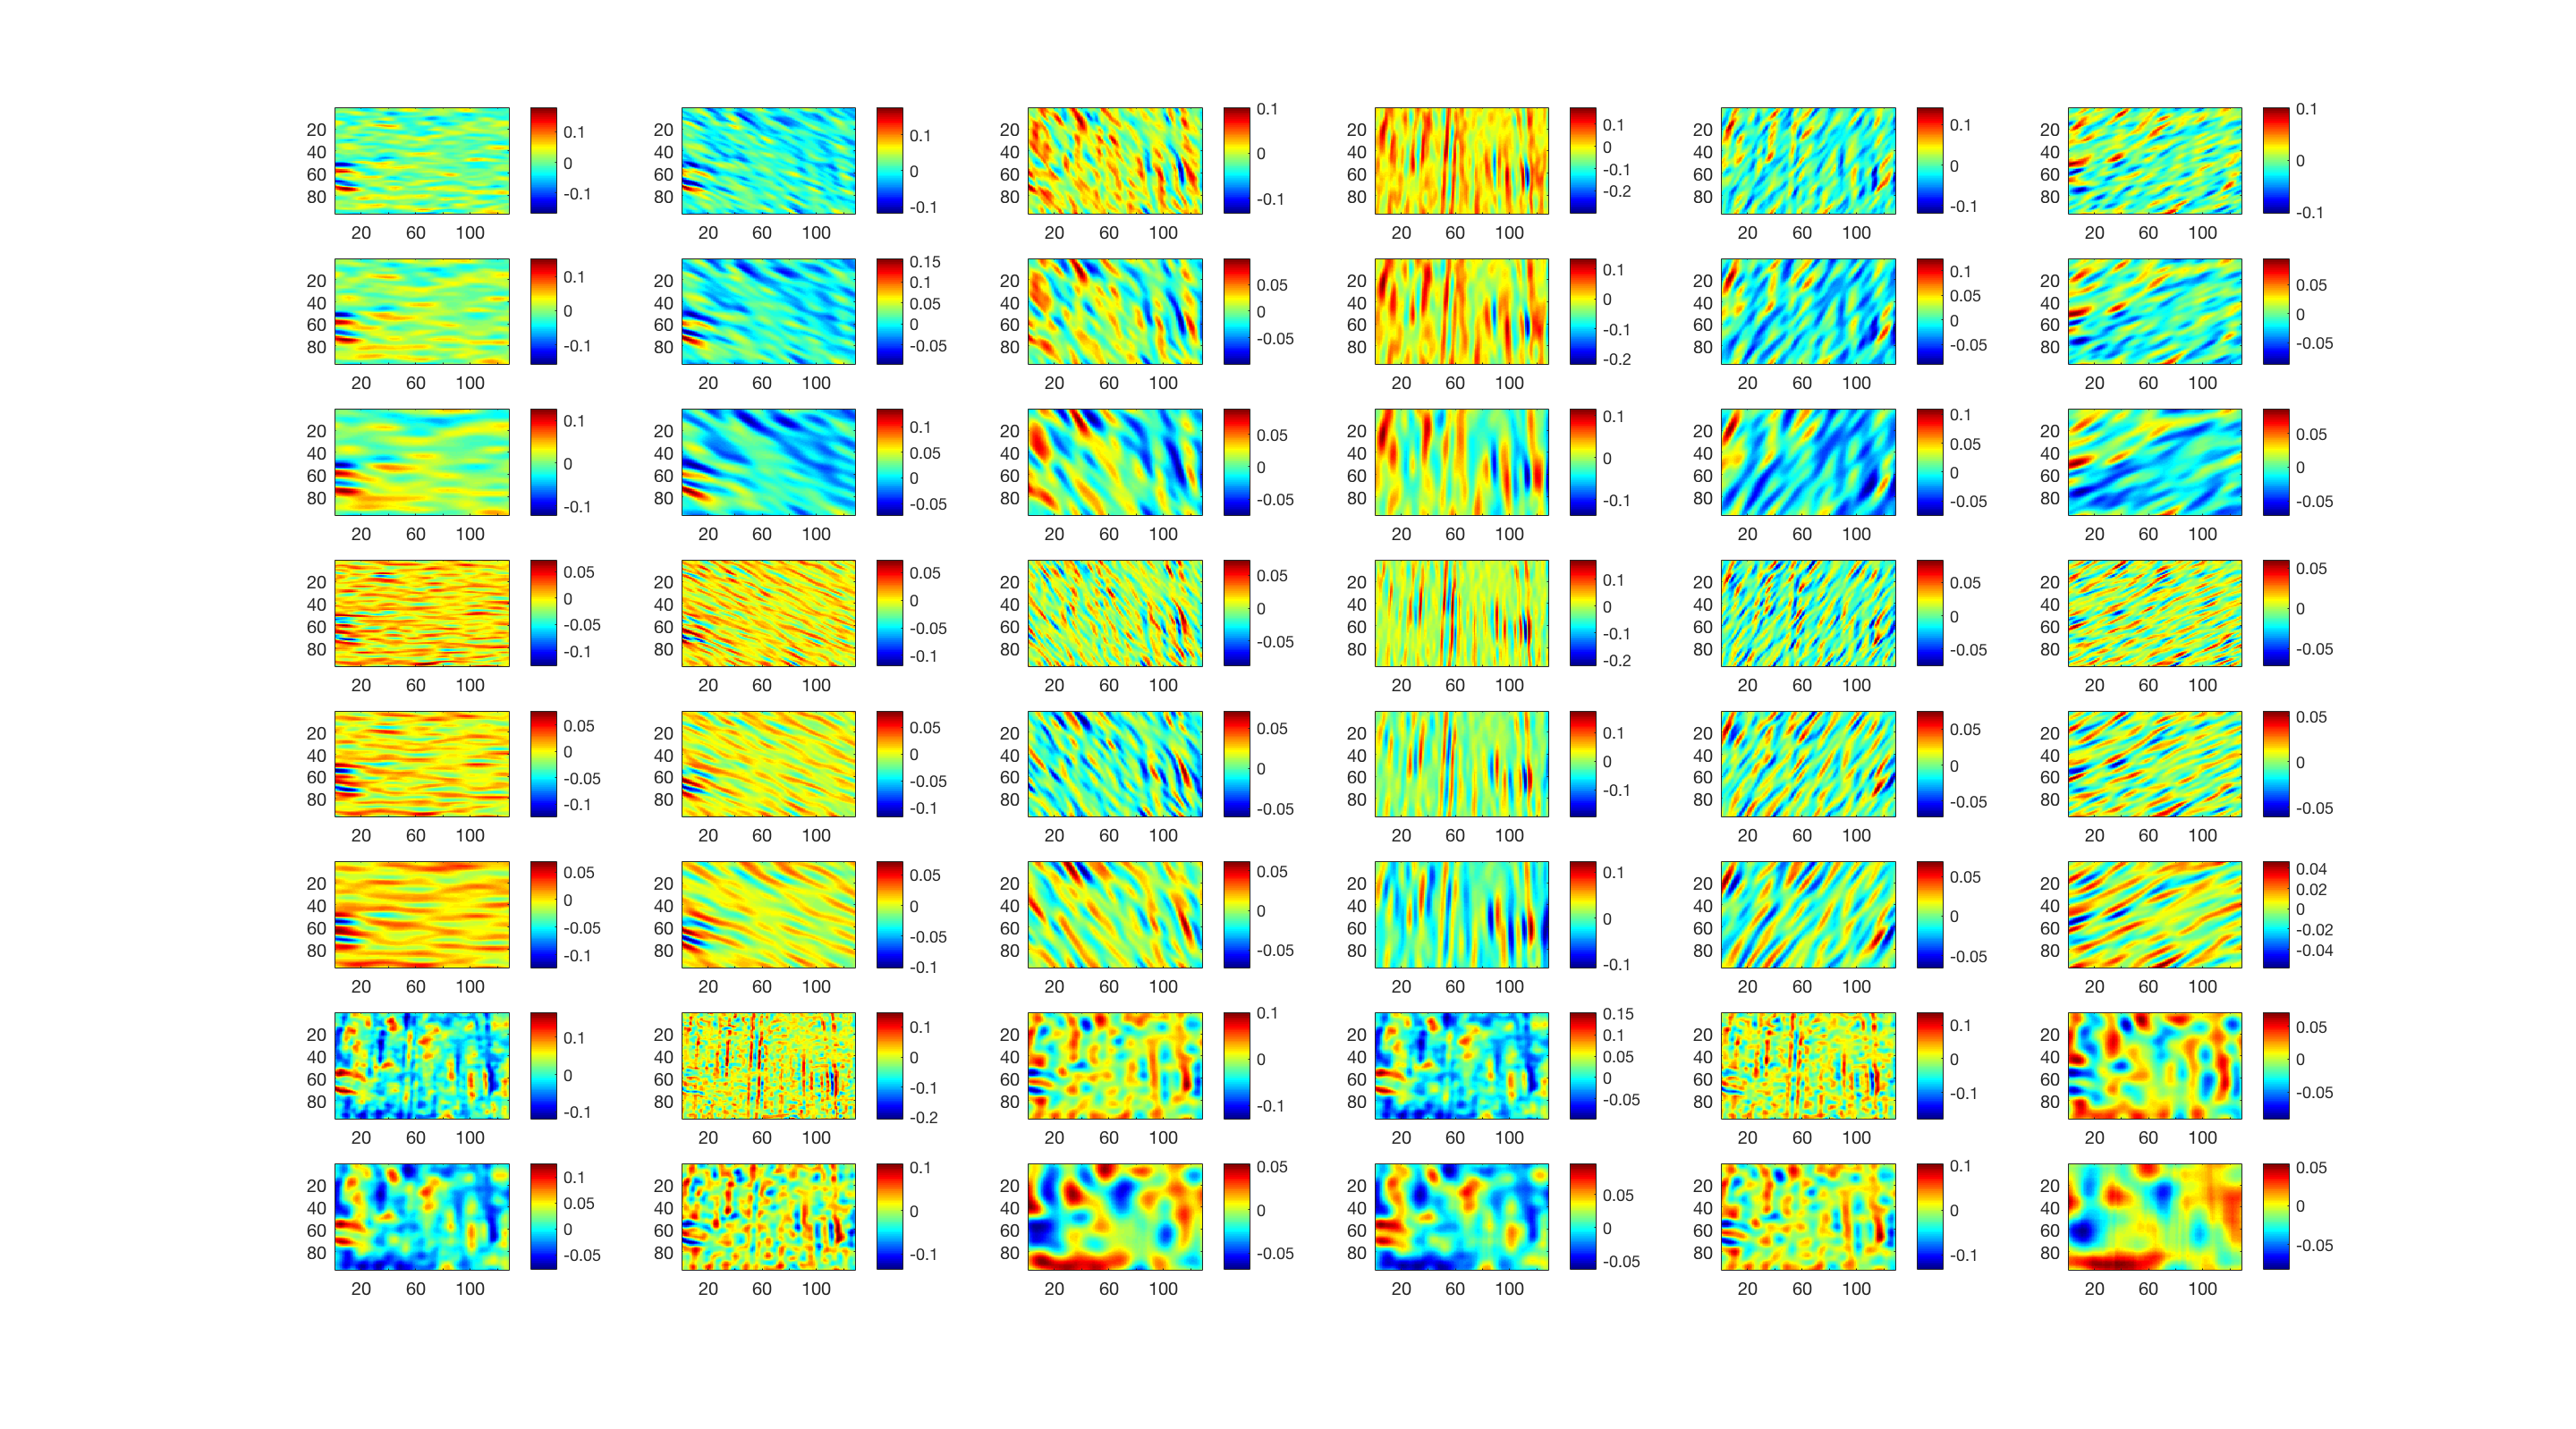
\includegraphics[width=0.9\textwidth]{img/f9_responses}
  \caption{Responses of \texttt{forest\_9} to the LM filter bank}
  \label{fig:f9ResponseB}
\end{figure}

Figure \ref{fig:f9ResponseC} normalizes the visualization of responses so they all lie on the same scale between the global minimum of $-0.2982$ and maximum of $0.1799$. It can be observed that the filters of vertical first gaussian derivatives get a strong result on this image, most probably caused by the edges of the vertical tree trunks. The responses for filters with a horizontal orientation on the other hand are much lower.

\begin{figure}[!hbt]
  \centering
  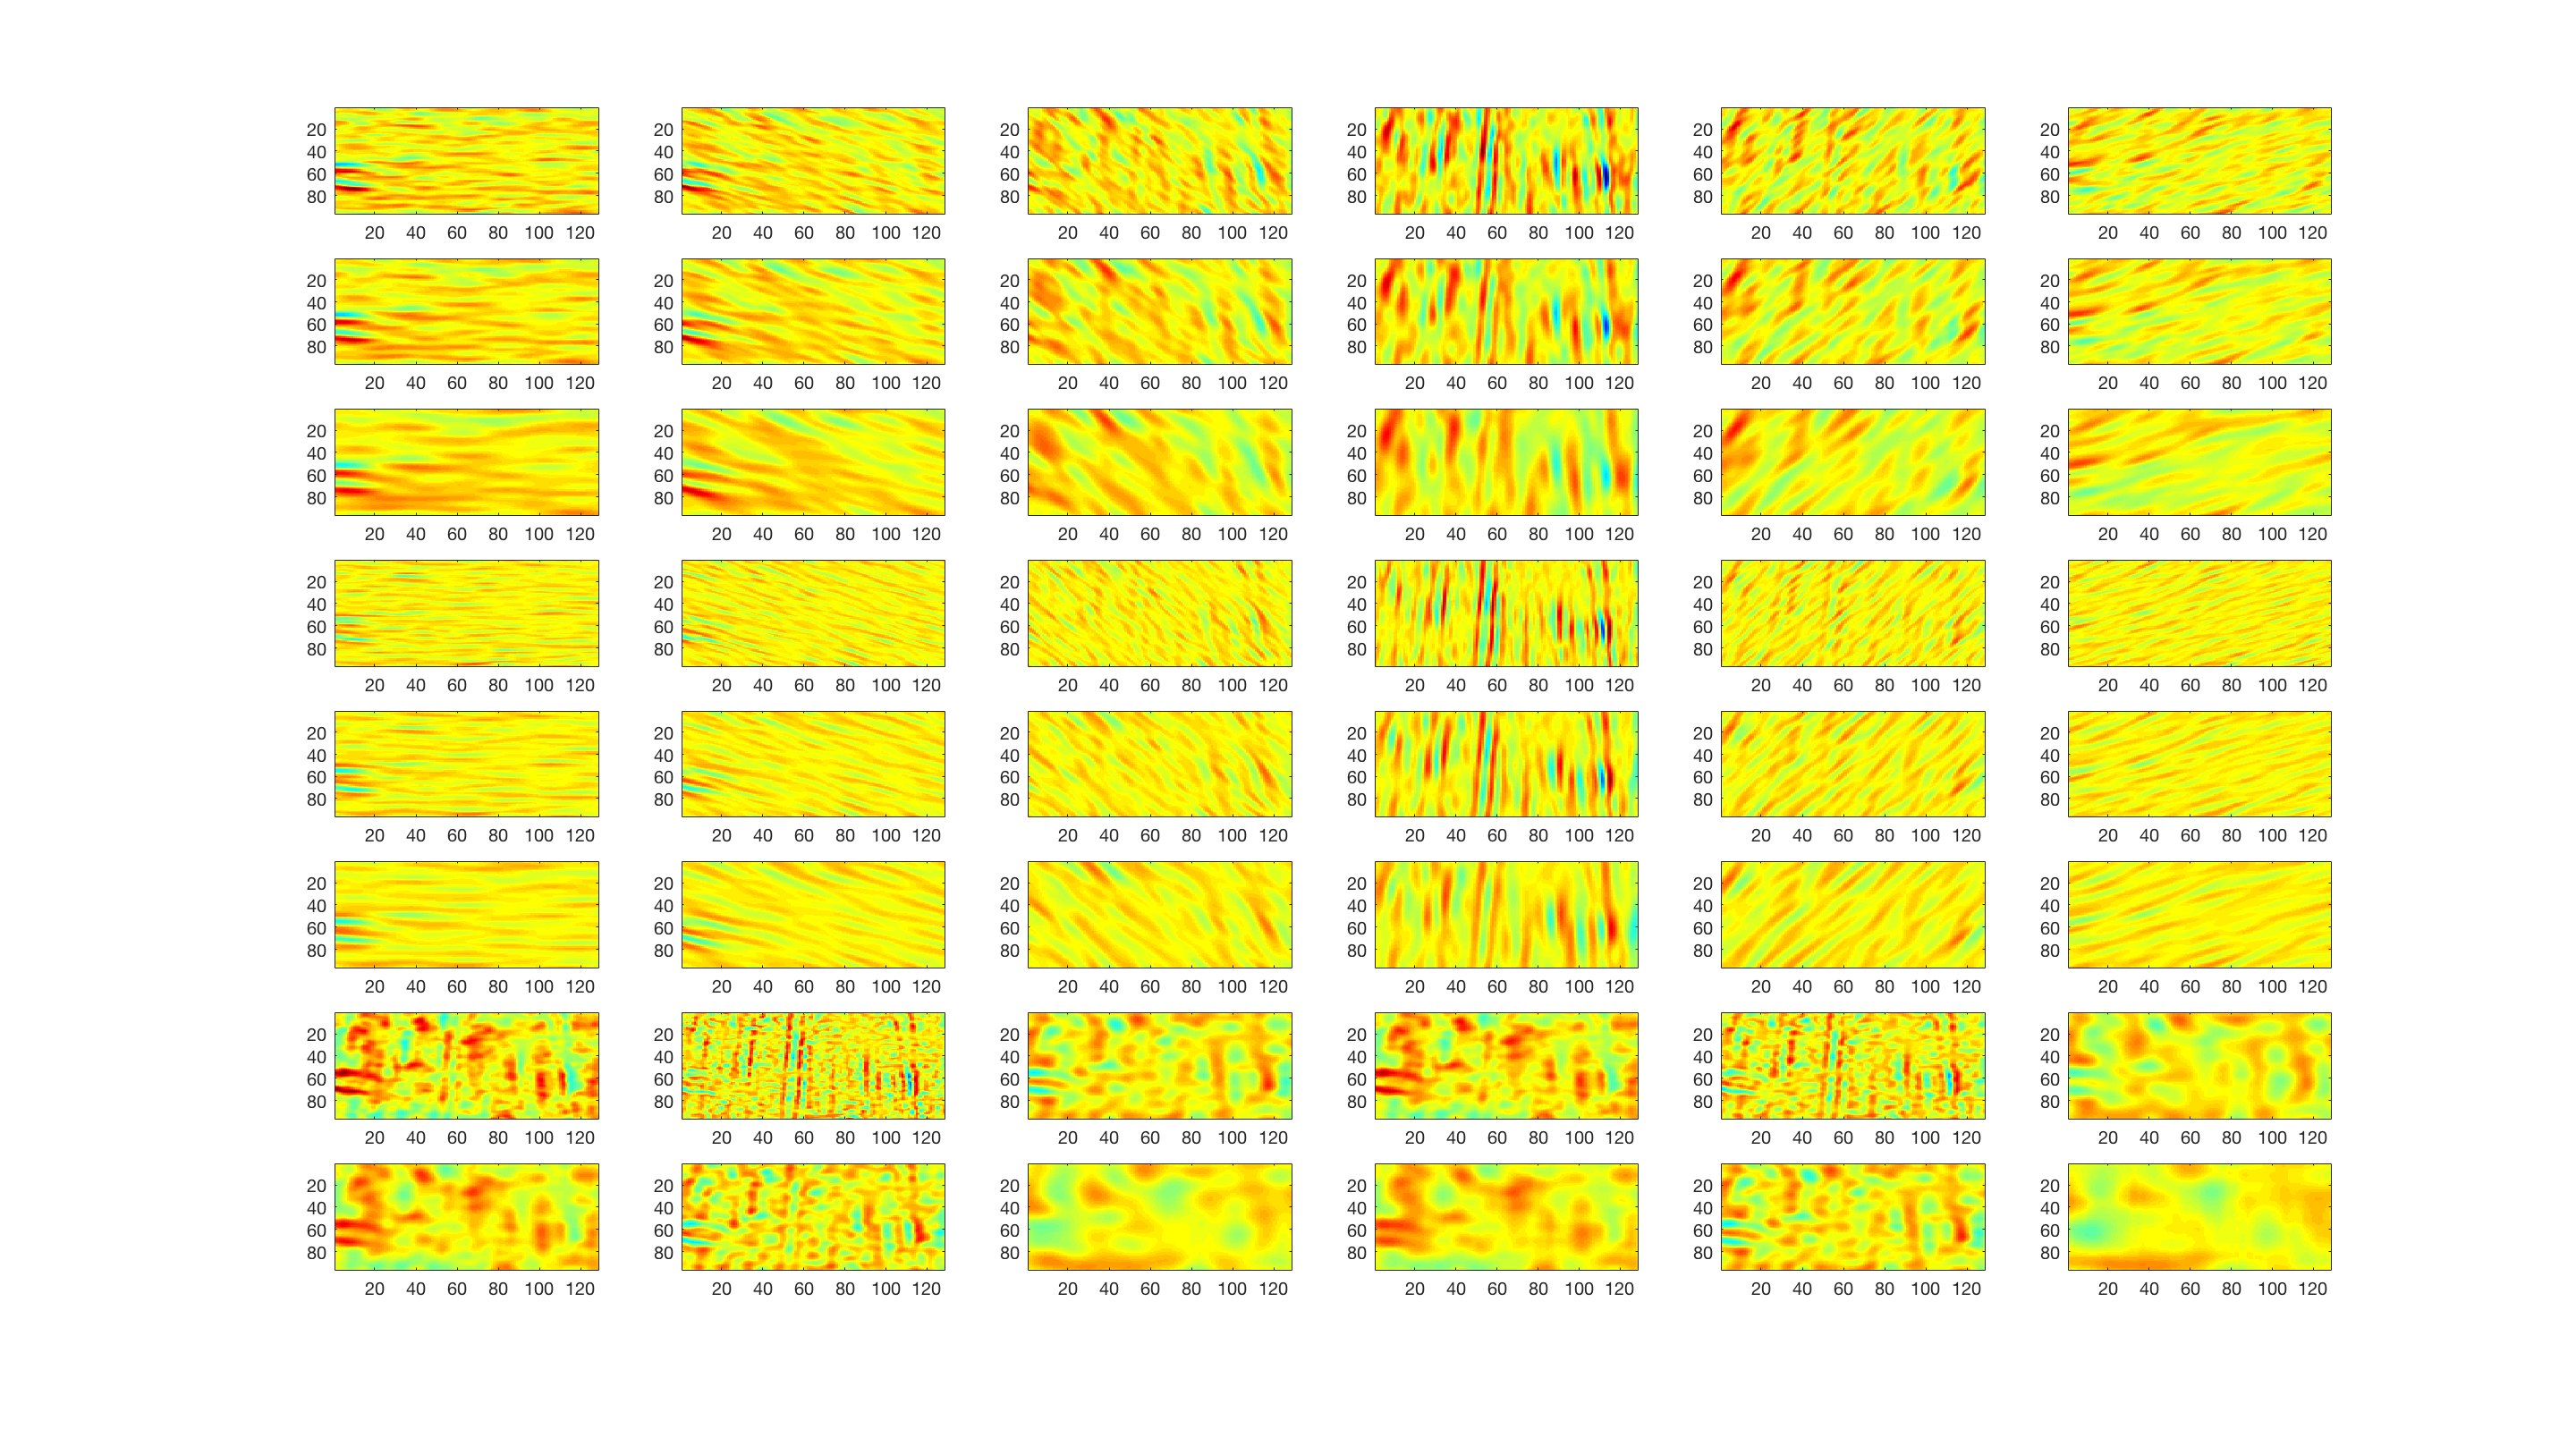
\includegraphics[width=0.9\textwidth]{img/f9_responses_normalized}
  \caption{Normalized responses of \texttt{forest\_9} to the LM filter bank.}
  \label{fig:f9ResponseC}
\end{figure}



As comparison to the forest scene, responses to \texttt{buildings\_2} (figure \ref{fig:b2ResponseA}) can be seen in figure \ref{fig:b2ResponseB}. Here, the slight diagonal filters yield a relatively high response. The responses clearly differ between the image of the forest and the image of a building. The first derivatives of gaussians yield a high response along the edges of the building. 

\begin{figure}[!hbt]
  \centering
  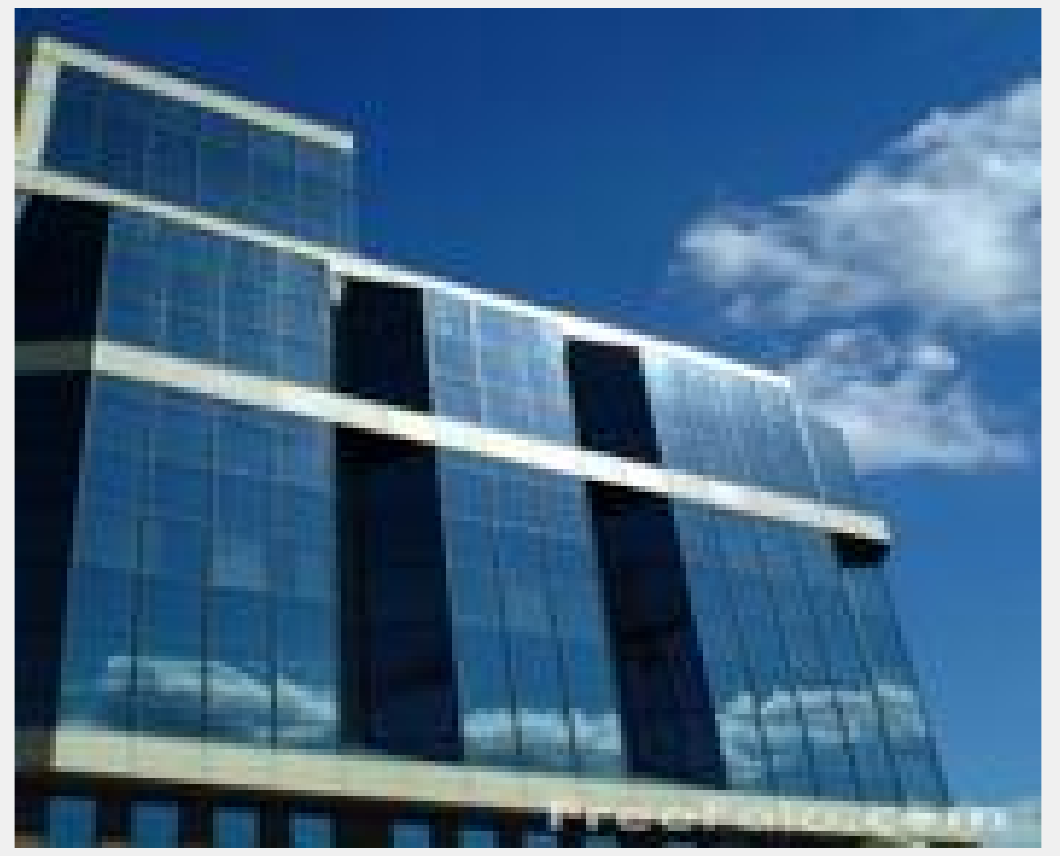
\includegraphics[width=0.4\textwidth]{img/b2}
  \caption{Example image \texttt{buildings\_2}}
  \label{fig:b2ResponseA}
\end{figure}

\begin{figure}[!hbt]
  \centering
  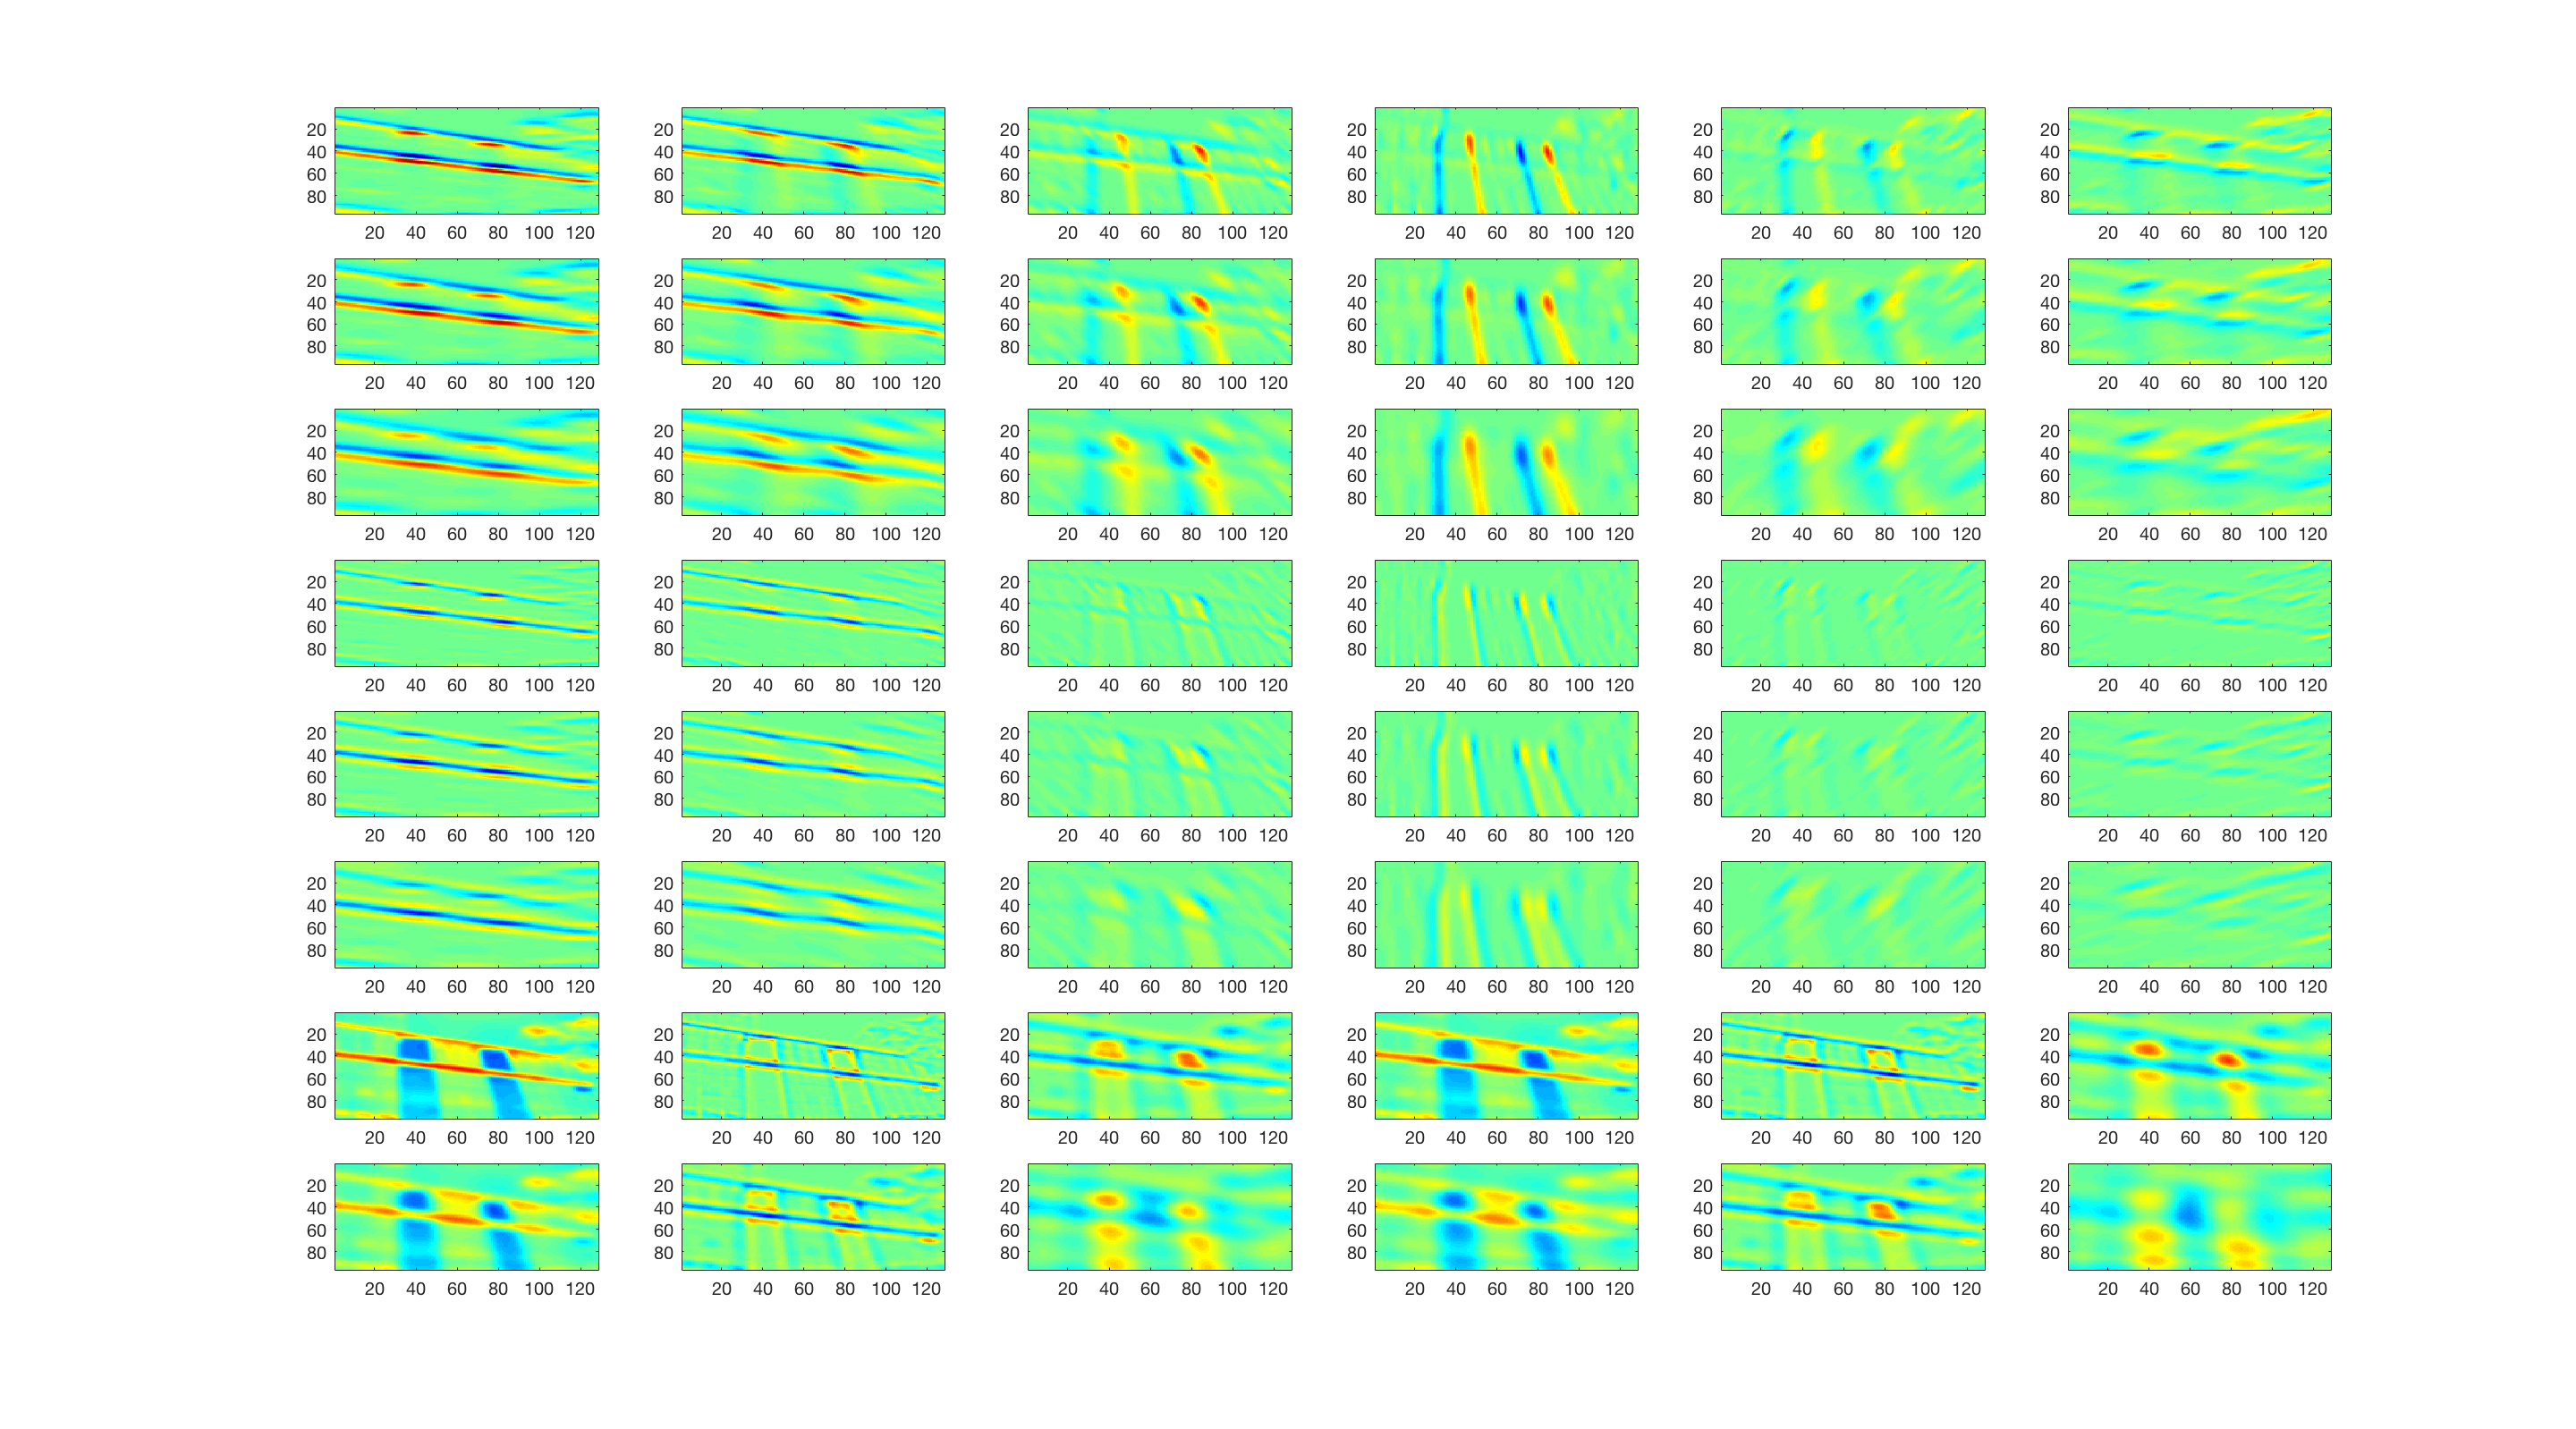
\includegraphics[width=0.9\textwidth]{img/b2_responses_normalized}
  \caption{Normalized responses of \texttt{buildings\_2} to the LM filter bank}
  \label{fig:b2ResponseB}
\end{figure}

To evaluate the difference of responses between the different classes of images more quantitatively, we examined the boxplots of the responses showing mean, standard deviation and range of values in figure \ref{fig:boxplots}. Subfigure (a) shows boxplots for all 48 filter's responses for the \texttt{forest\_9} and subfigure (b) the corresponding responses of \texttt{buildings\_2}. It can be seen easily, that the responses have a very different distribution of values for the two images.

\begin{figure}[!hbt]
\centering
\subfigure[Responses for \texttt{forest\_9}]{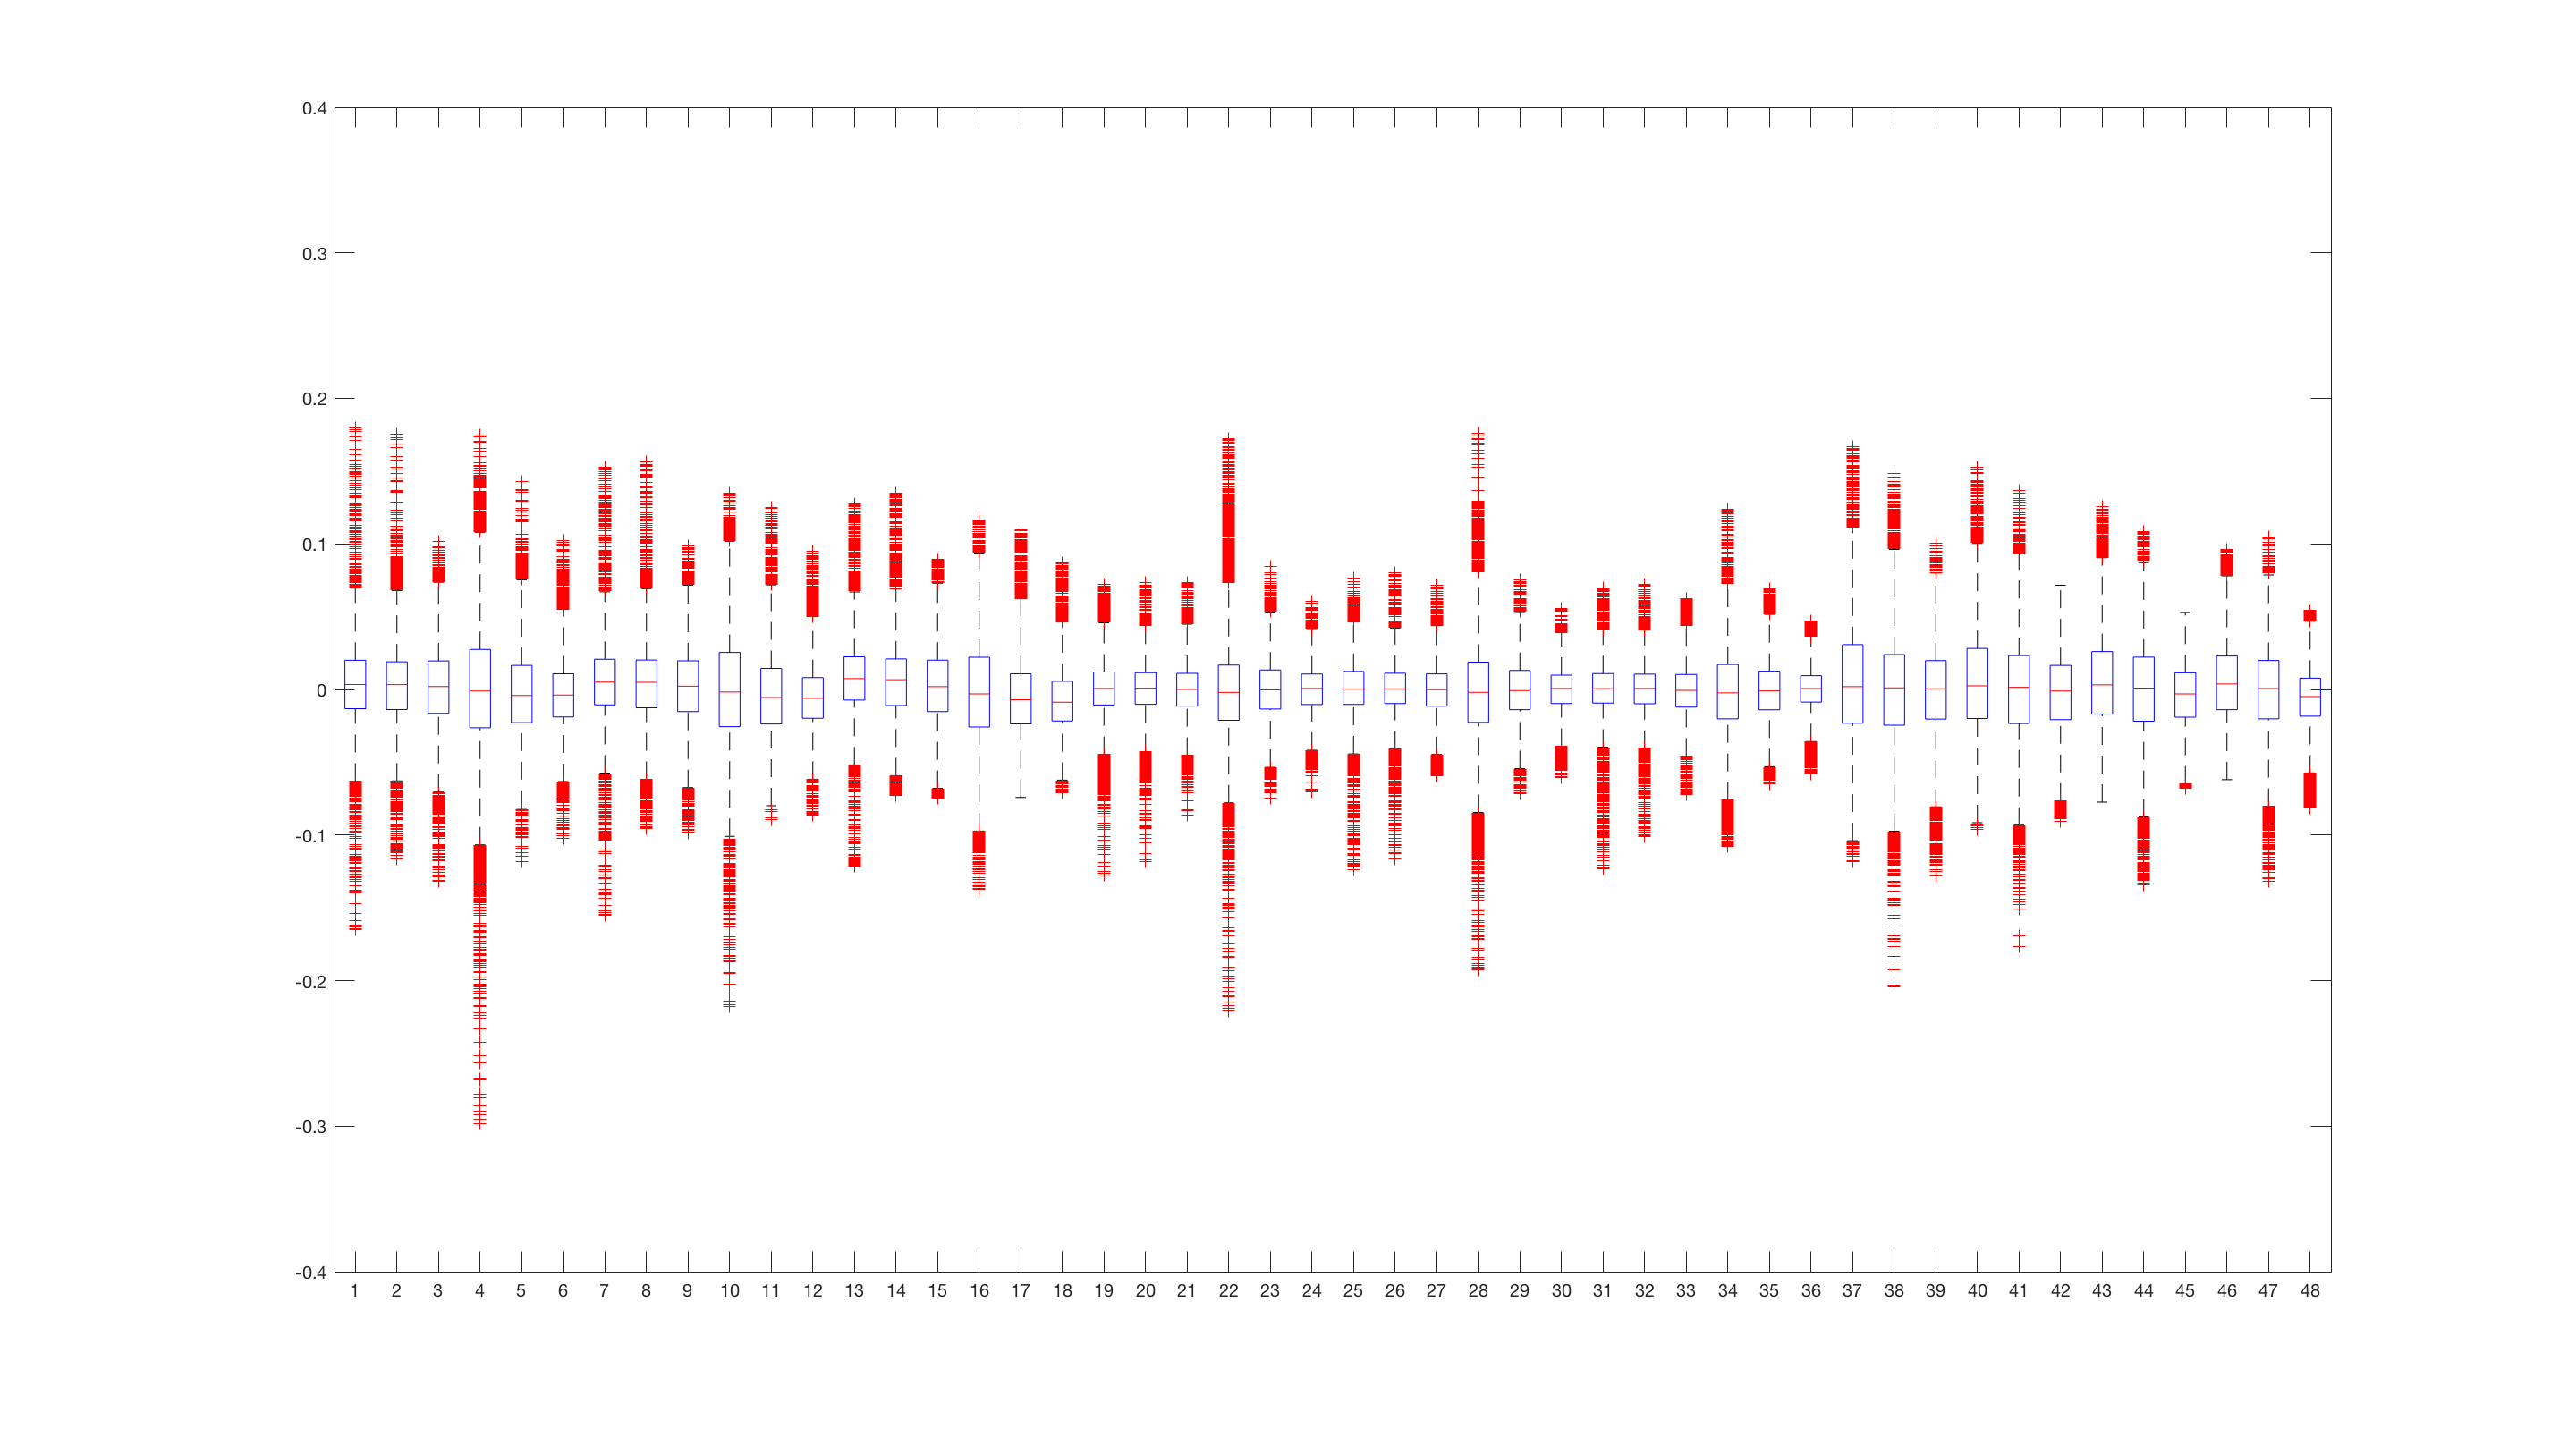
\includegraphics[width=\textwidth]{img/f9_boxplots}} \\
\subfigure[Responses for \texttt{buildings\_2}]{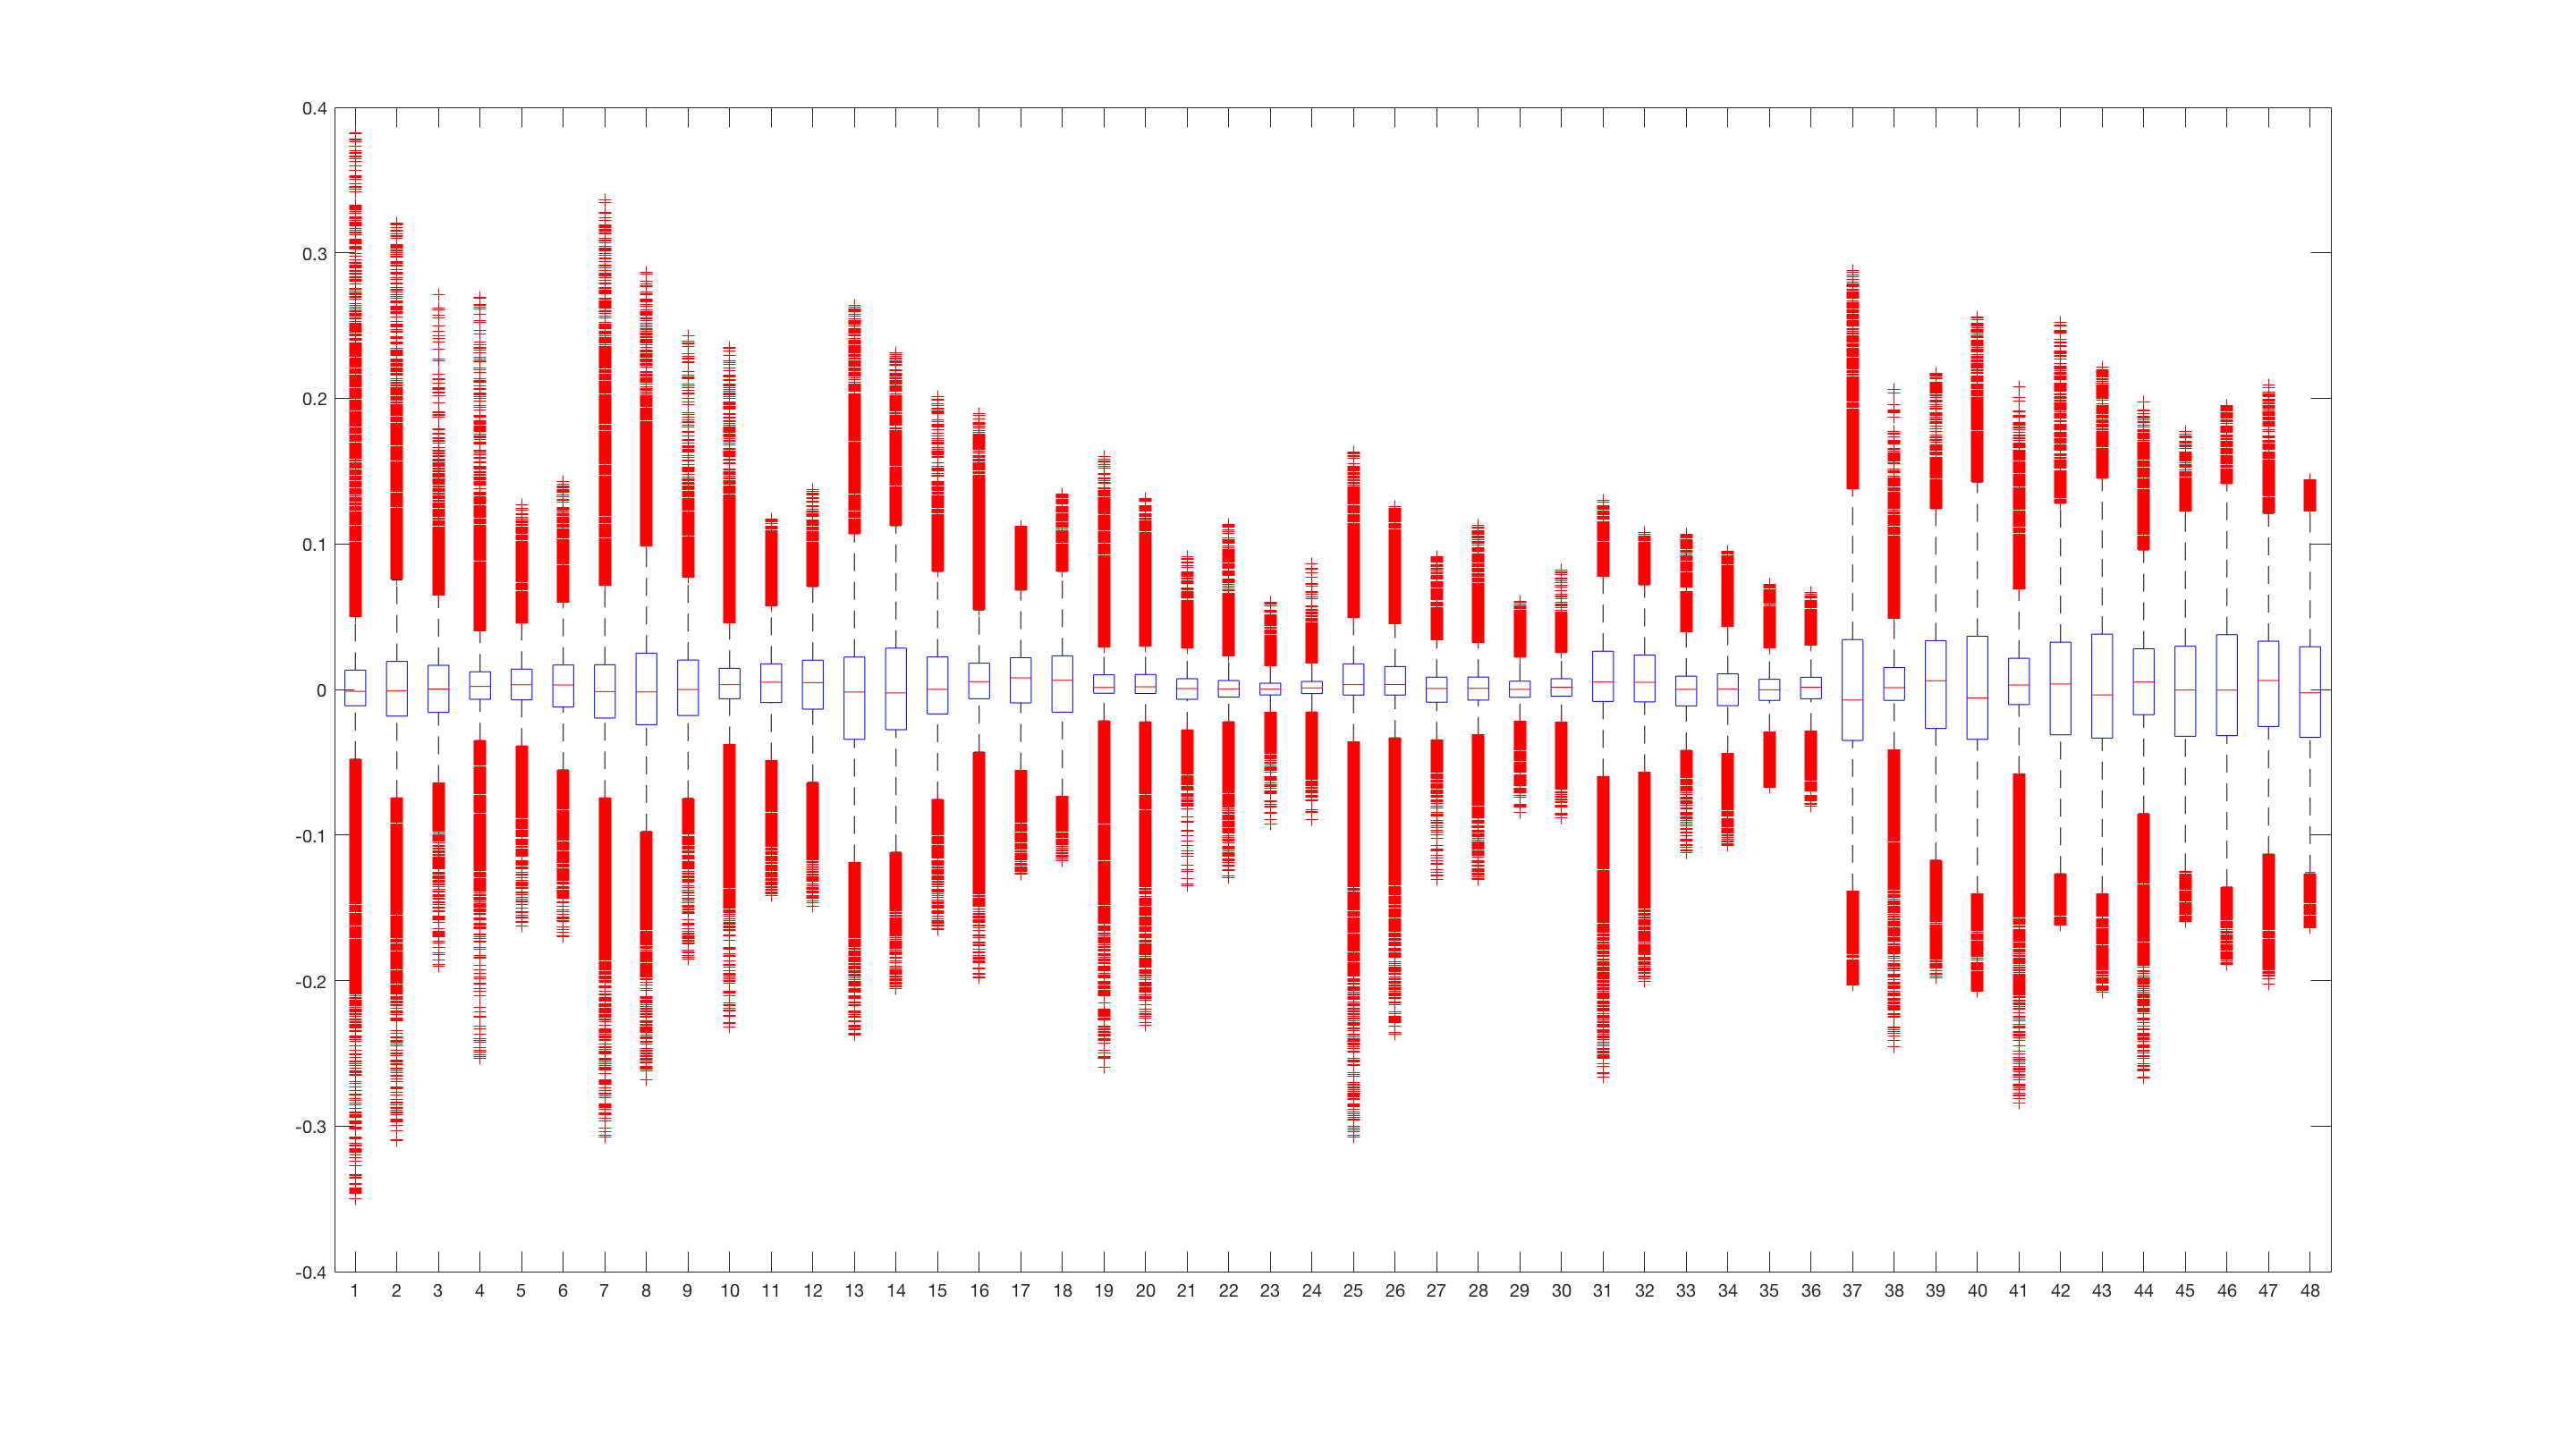
\includegraphics[width=\textwidth]{img/b2_boxplots}}
\caption{Boxplots of responses to LM filter bank}
\label{fig:boxplots}
\end{figure}

In figure \ref{fig:means} we show the differences of mean responses and standard deivation of the responses. Again, we can observe a quite unique distribution for both images.

\begin{figure}[!hbt]
\centering
\subfigure[Mean responses]{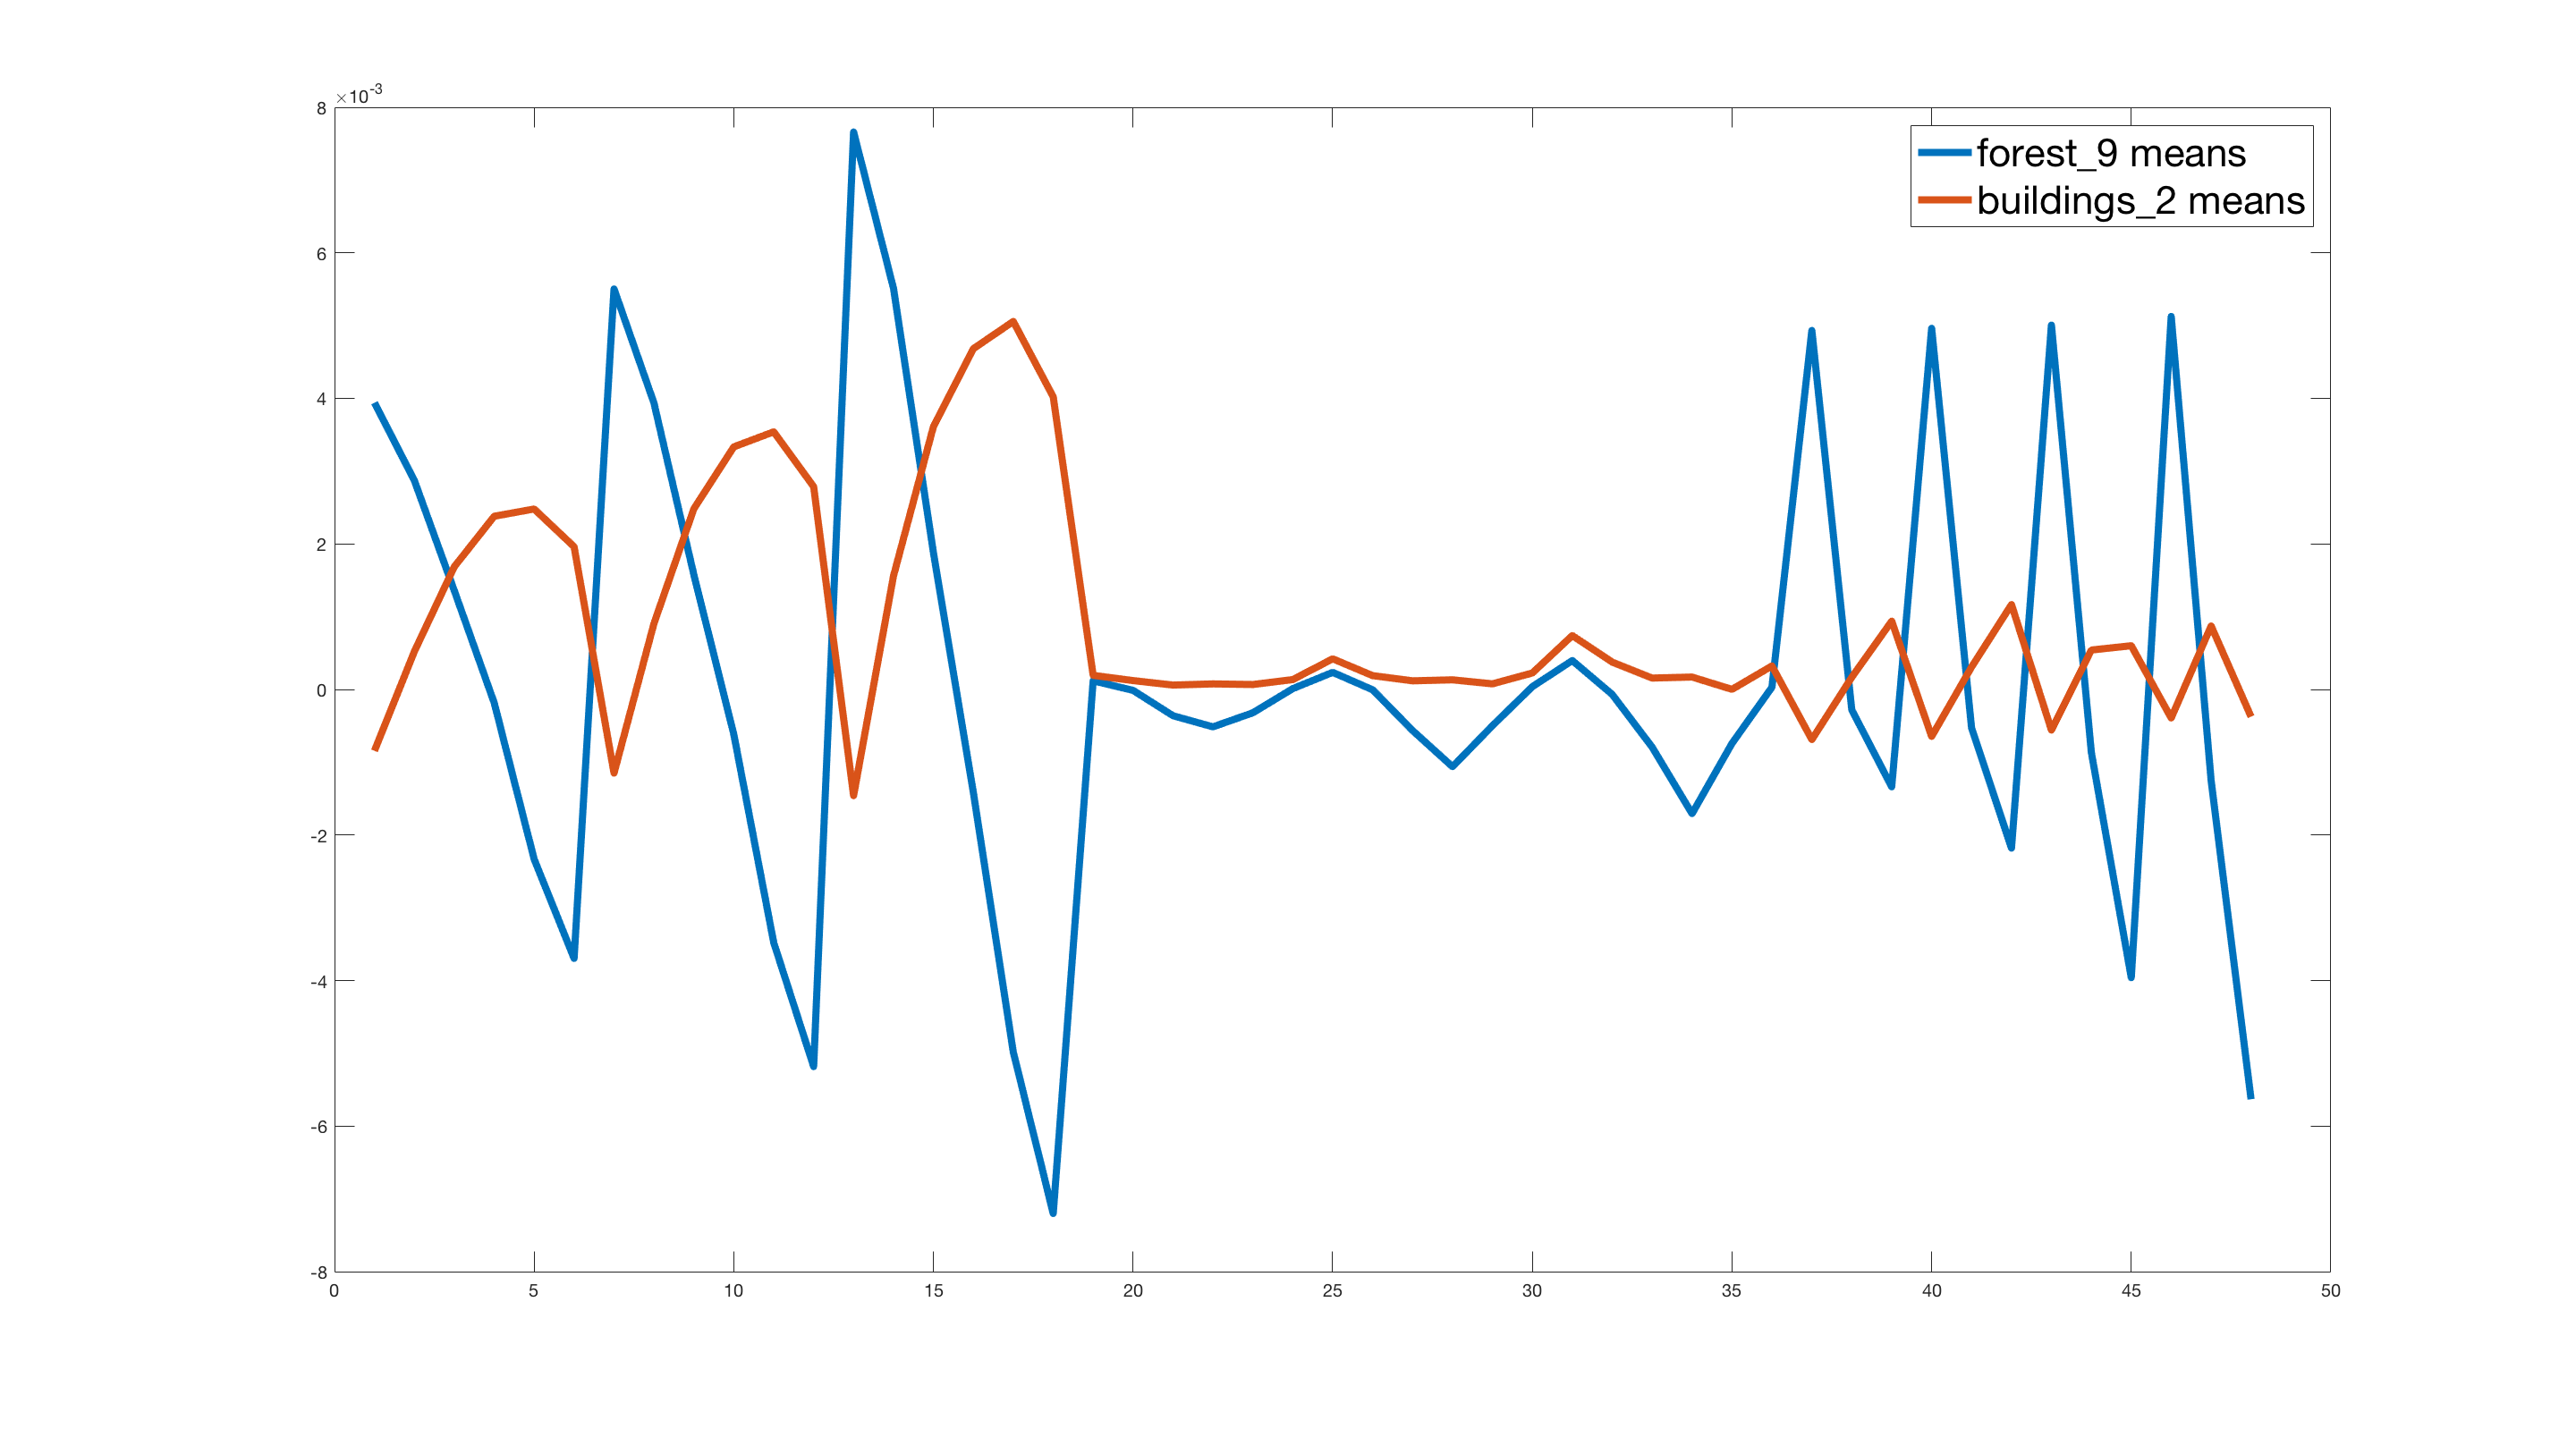
\includegraphics[width=0.45\textwidth]{img/f9b2_means}}
\subfigure[Standard deviation of responses]{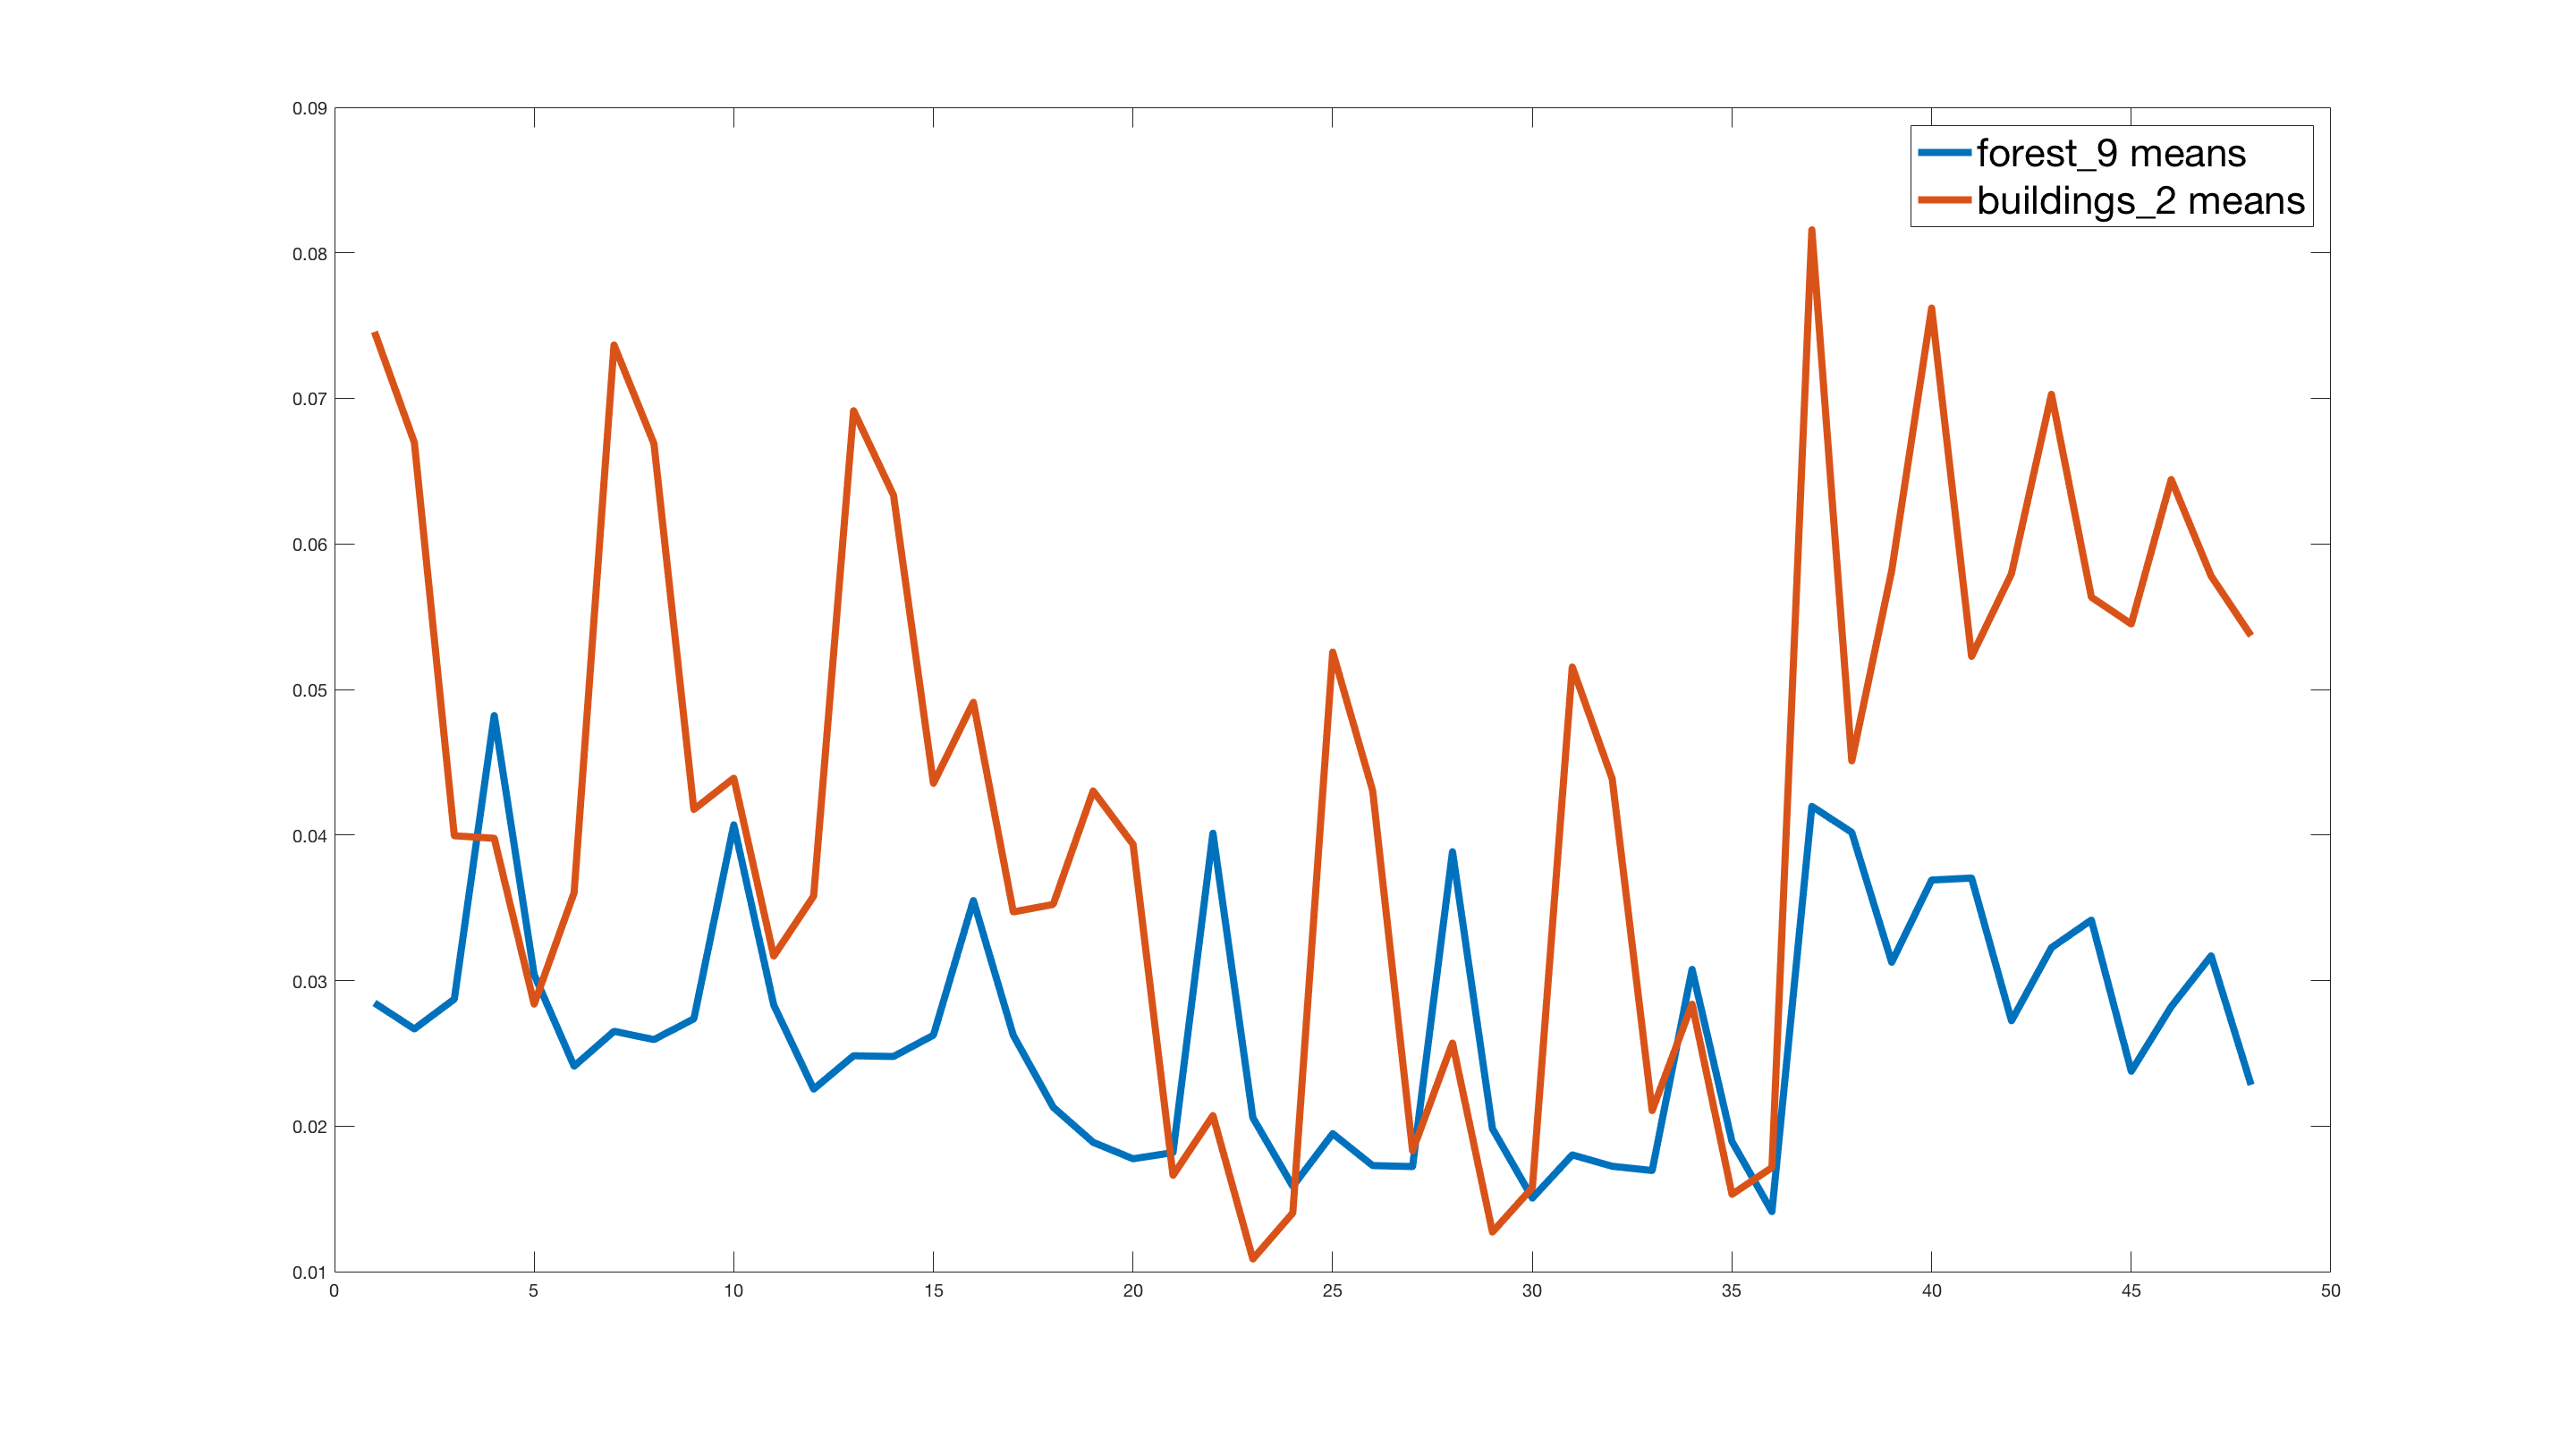
\includegraphics[width=0.45\textwidth]{img/f9b2_sds}}
\caption{Comparison of mean and standard deviation}
\label{fig:means}
\end{figure}

\section{Class Feature Matrices}

When applying the convolutions of the LM filter bank, responses for the filters are usually different in different parts of an image. In order to describe an image's texture with a small but expressive number of descriptors, we need to aggregate the responses of the image for each filter into single values. For this we can calculate descriptive metrics such as mean, standard deviation, or median. For example, the mean response for the first filter will be one feature, the mean response for the second filter another one, and so on. We construct a feature matrix for each class (forest, buildings, and sunset) of images with each row corresponding to an image and each column corresponding to the aggregated response of this image to a filter of the LM filter bank. In the following sections we explored the following aggregations: mean, standard deviation, minimum, maximum, and median.
As we show in section \ref{sec:vis1}, not all aggregations lead to the same separability of the different classes of images. Our experiments showed, for example, that the class of sunset images can be distinguished best from other classes when looking comparing the standard deviations of results. 


\section{Visualizing Class Feature Differences}
\label{sec:vis1}

For each image we obtain a vector of aggregated responses for each filter of the LM filter bank. In this section we show some examples of how well these descriptors are able to be used to separate the classes.
Figure \ref{fig:m41_m25} plots the mean values of filter 41 (x-axis) and filter 25 (y-axis) for all 90 images. Green dots correspond to forest images, blue dots to buildings and red dots to sunsets (this color code is used through the entire report). The classes are clearly not linearly separable based on these two features alone. There also is no obvious and elegant non-linear separation. 

\begin{figure}[!hbt]
  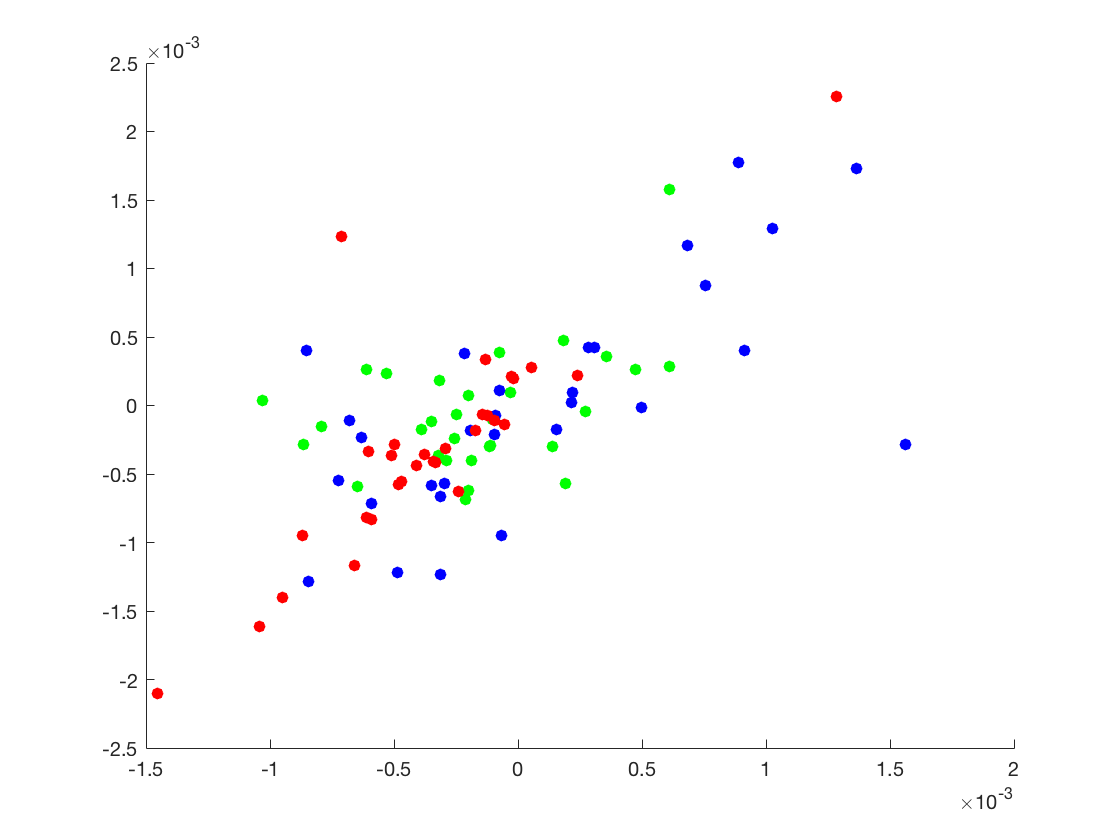
\includegraphics[width=\textwidth]{img/m41_m25}
    \caption{Mean responses to filter 41 and filter 25}
  \label{fig:m41_m25}
\end{figure}

Figure \ref{fig:sd41_sd25} compares the standard deviations of the responses to the same filters, 41 on the x-axis and 25 on the y-axis. We can see here, that the classes are much better separable. Especially the sunset class tends to have a higher standard deviation of the filter 25 response and can - ignoring some outliers - be separated linearly. The building and forest class lie more closely together, but even here a non-linear separation can be assumed. For these two filters, standard deviation seems to be a better aggregation to separate the different classes.

\begin{figure}[!hbt]
  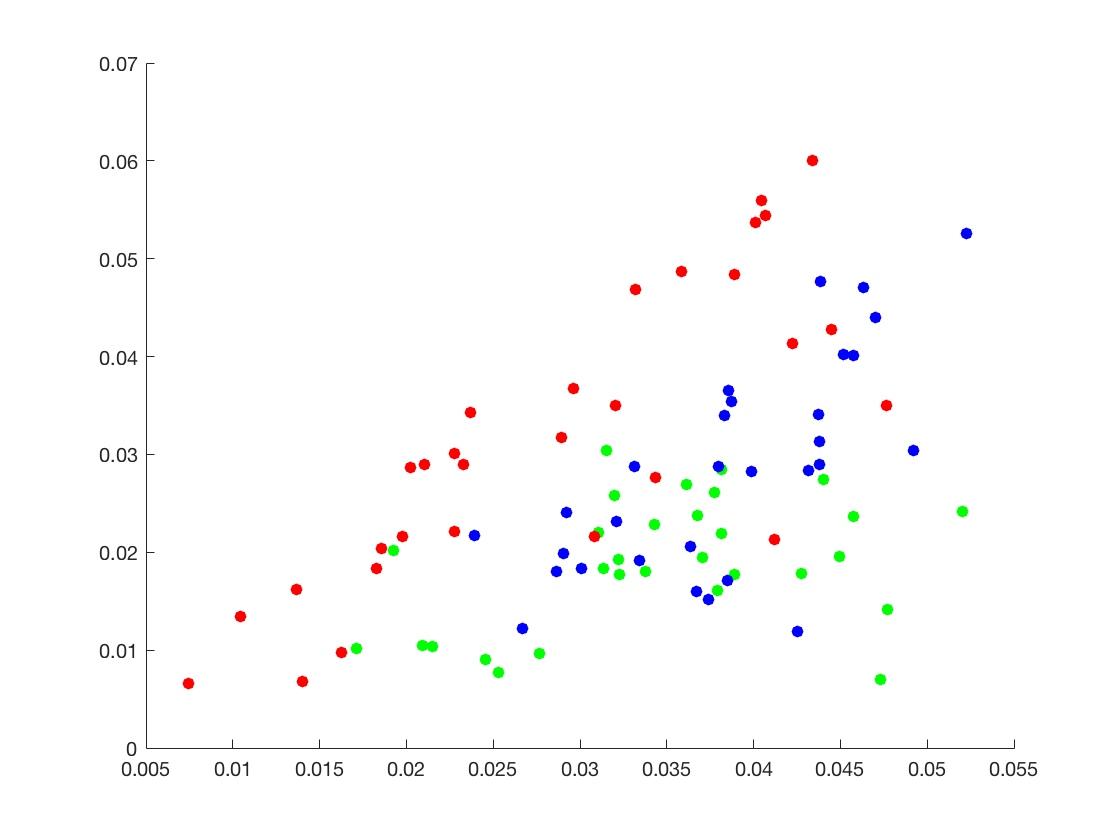
\includegraphics[width=\textwidth]{img/sd41_sd25}
    \caption{Standard deviation of responses to filter 41 and filter 25}
  \label{fig:sd41_sd25}
\end{figure}

Another good result can be seen when comparing the mean of responses to filter 21 (x-axis) to the standard deviation of responses to the same filter (y-axis) in figure \ref{fig:m21_sd21}. Like in the previous example, the sunset class is more distinguished from the two other classes. 

\begin{figure}[!hbt]
  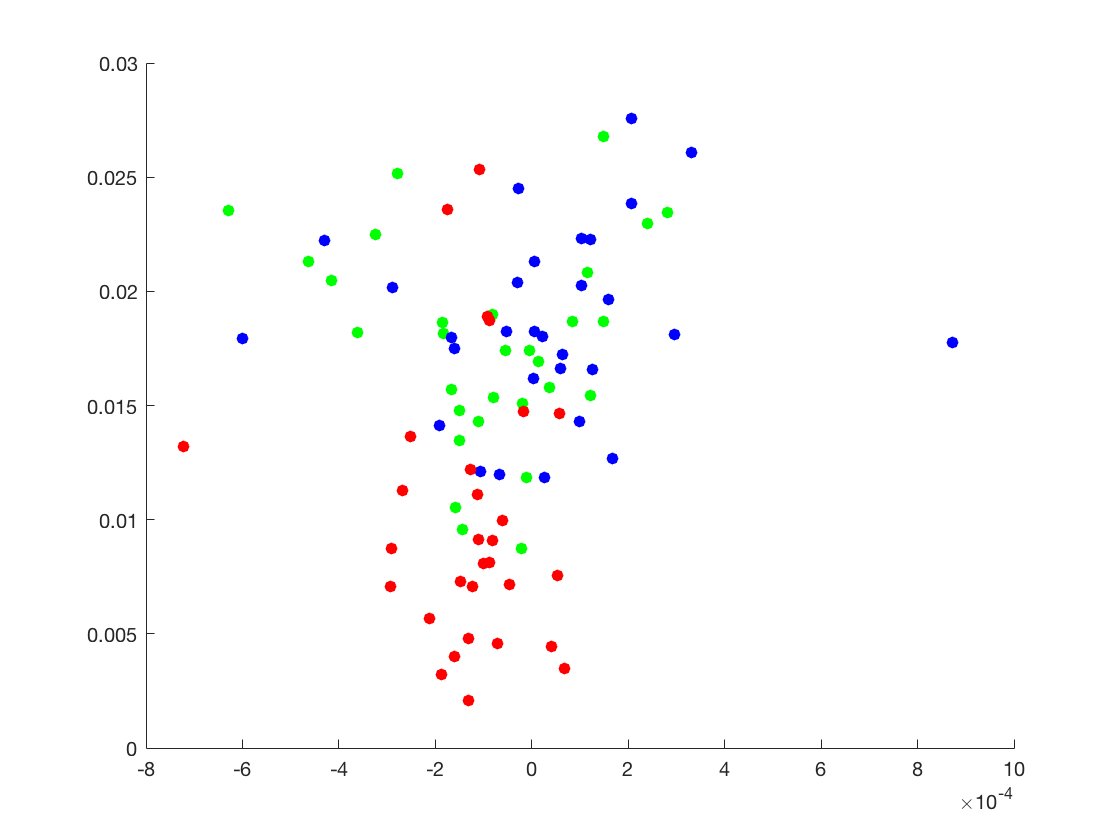
\includegraphics[width=\textwidth]{img/m21_sd21}
    \caption{Mean and standard deviation of responses to filter 21}
  \label{fig:m21_sd21}
\end{figure}

\section{KNN Search for Similar Images}

The objective of this report is to evaluate the capabilities of texture features for retrieving images that are most similar to a queried image. For this, we use a knn (k nearest neighbors) search algorithm that returns the 9 images whose features are most similar to the given image, using euclidean distance to quantify similarity. 

In figure \ref{fig:100000} we show the results of retrieving 9 similar images for both \texttt{forest\_9} and \texttt{building\_5} when using only the means of responses as features. The retrieved images are sorted by similarity from top left to bottom right. 

\begin{figure}[!hbt]
\centering
\subfigure[\texttt{forest\_9}]{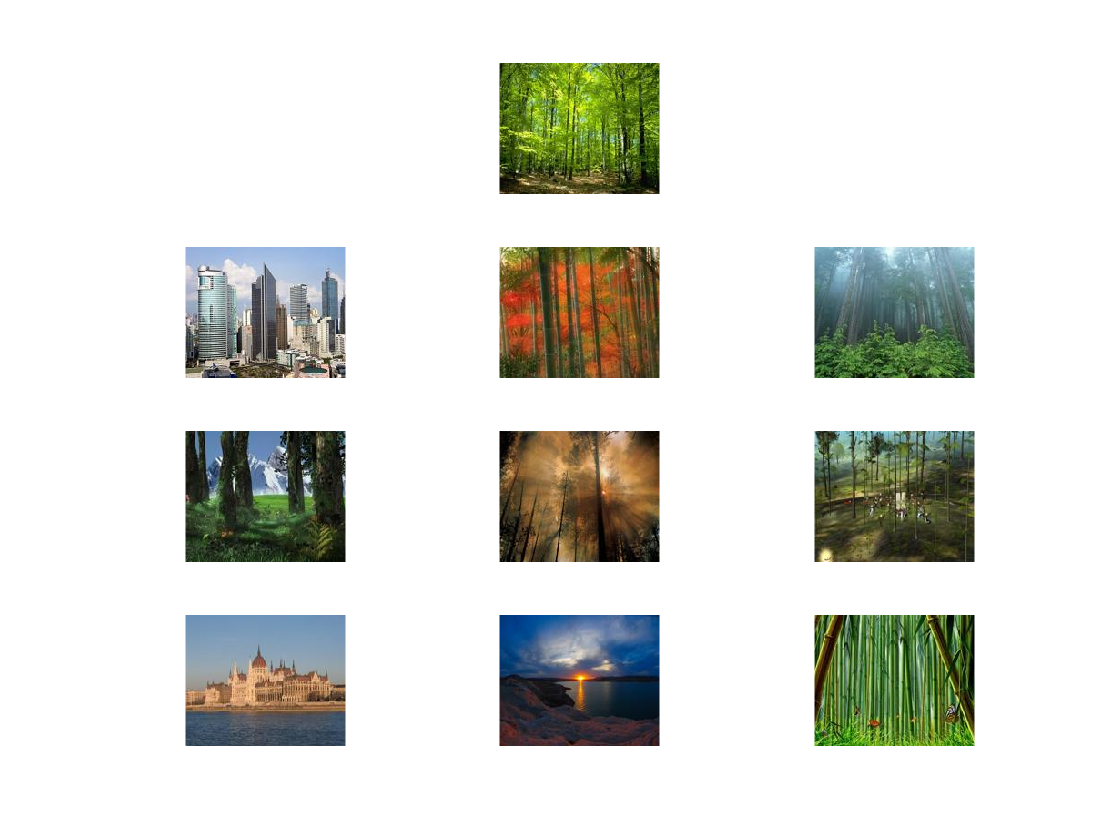
\includegraphics[width=0.45\textwidth]{img/f9knn_100000}}
\subfigure[\texttt{buildings\_5}]{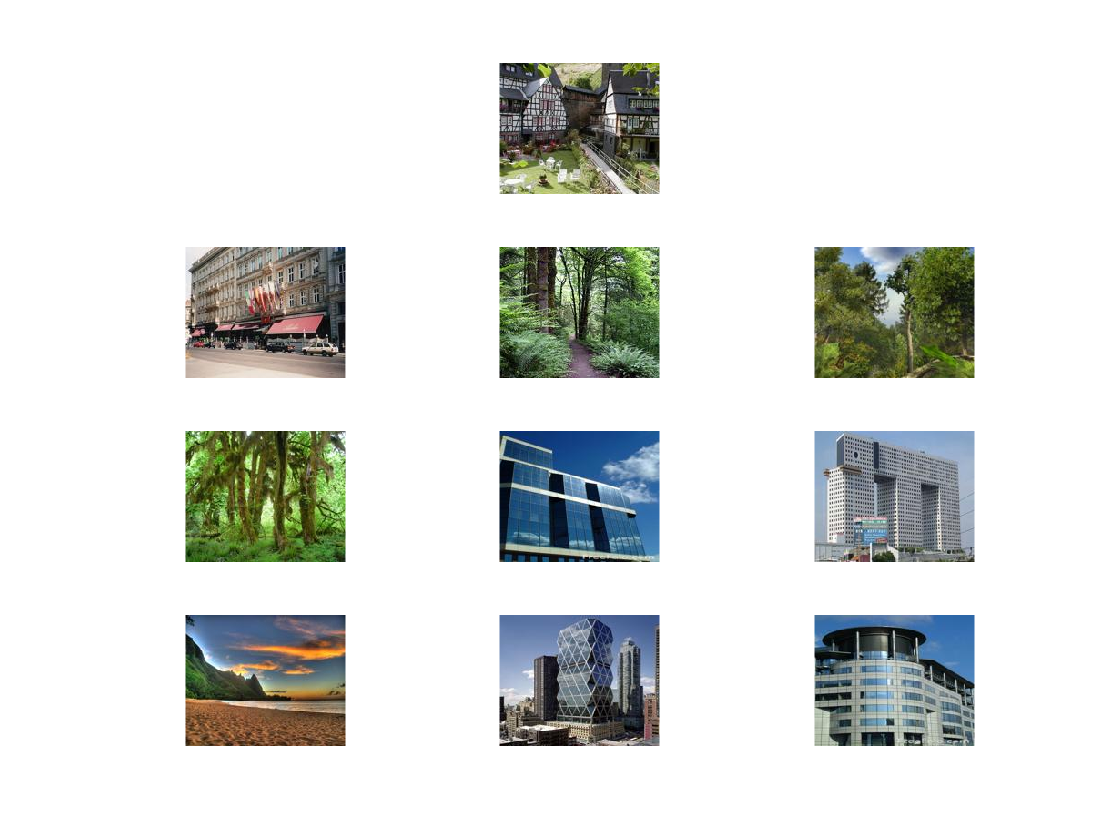
\includegraphics[width=0.45\textwidth]{img/b5knn_100000}}
\caption{Example KNN results for mean based features}
\label{fig:100000}
\end{figure}

We can see that the algorithm does succeed with retrieving some similar images, but also fails in some cases. For the forest image the result does contain a majority of other forest images, but the most similar image falsely is an image of a skyline and there is also an image of a sunset. The image \texttt{building\_5} is a bit more ambiguous, since it depicts both buildings but also grass and bushes that might have a similar texture to forest images. The results support this suspicion, consisting of a mix of forest and building images.

In figure \ref{fig:010000} we see the results for using standard deviation of filter responses as features. The results clearly improve over the ones obtained by using means as aggregation. Especially for the forest example, the top images are now all very similar forest landscapes. For the building example we still get a mix of forest and building images, but the sunset example disappeared.

\begin{figure}[!hbt]
\centering
\subfigure[\texttt{forest\_9}]{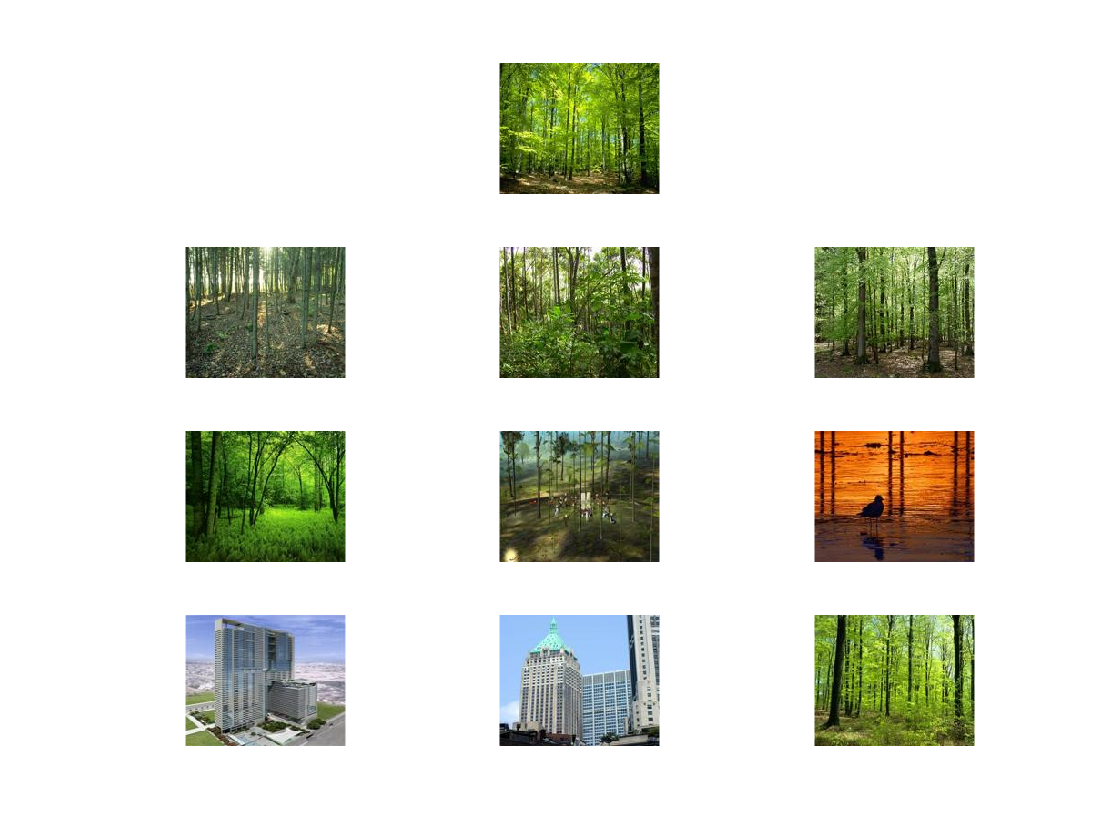
\includegraphics[width=0.45\textwidth]{img/f9knn_010000}}
\subfigure[\texttt{buildings\_5}]{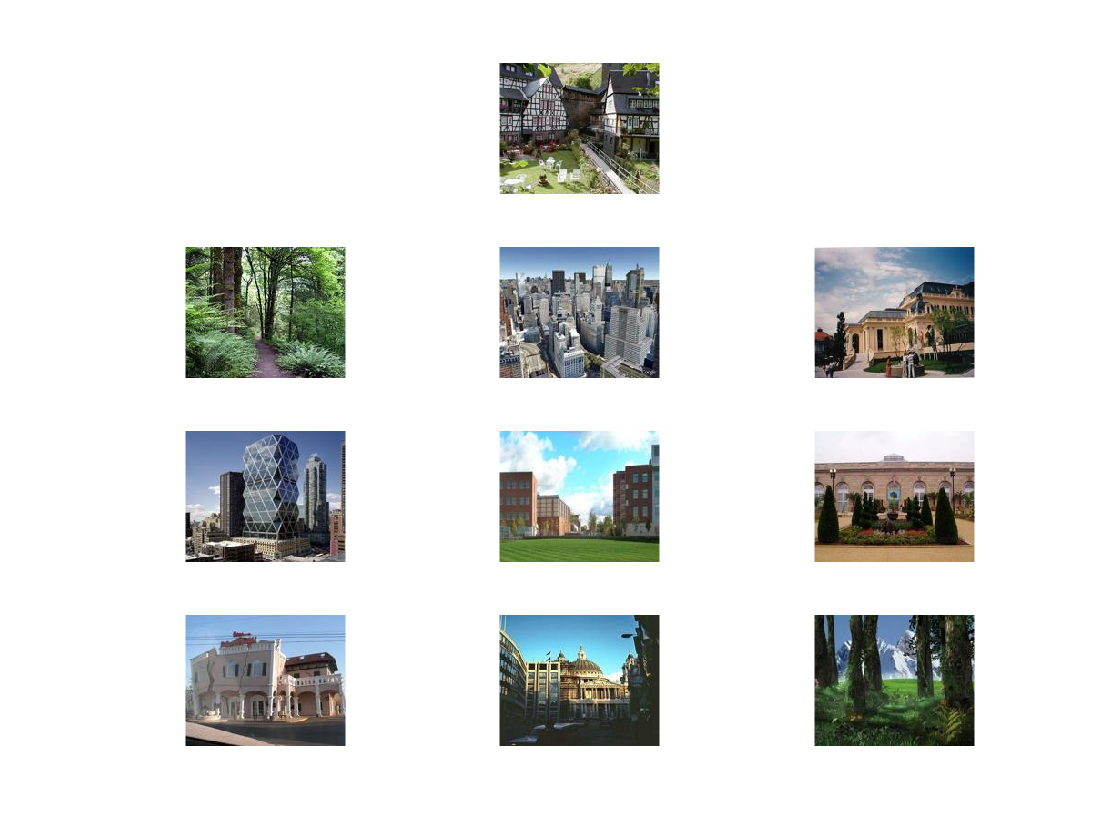
\includegraphics[width=0.45\textwidth]{img/b5knn_010000}}
\caption{Example KNN results for standard deviation based features}
\label{fig:010000}
\end{figure}

Figure \ref{fig:111110} shows the results when using all aggregations methods at once and building a big feature matrix consisting of means, standard deviations, minima, maxima and medians. The results seem to decrease in quality when using all features combined - possibly due to the ``curse of dimensionality'' when using distance functions in high dimensional spaces. Some sort of feature selection would be necessary here to improve the results again. This, however, was beyond the scope of this report. 

\begin{figure}[!hbt]
\centering
\subfigure[\texttt{forest\_9}]{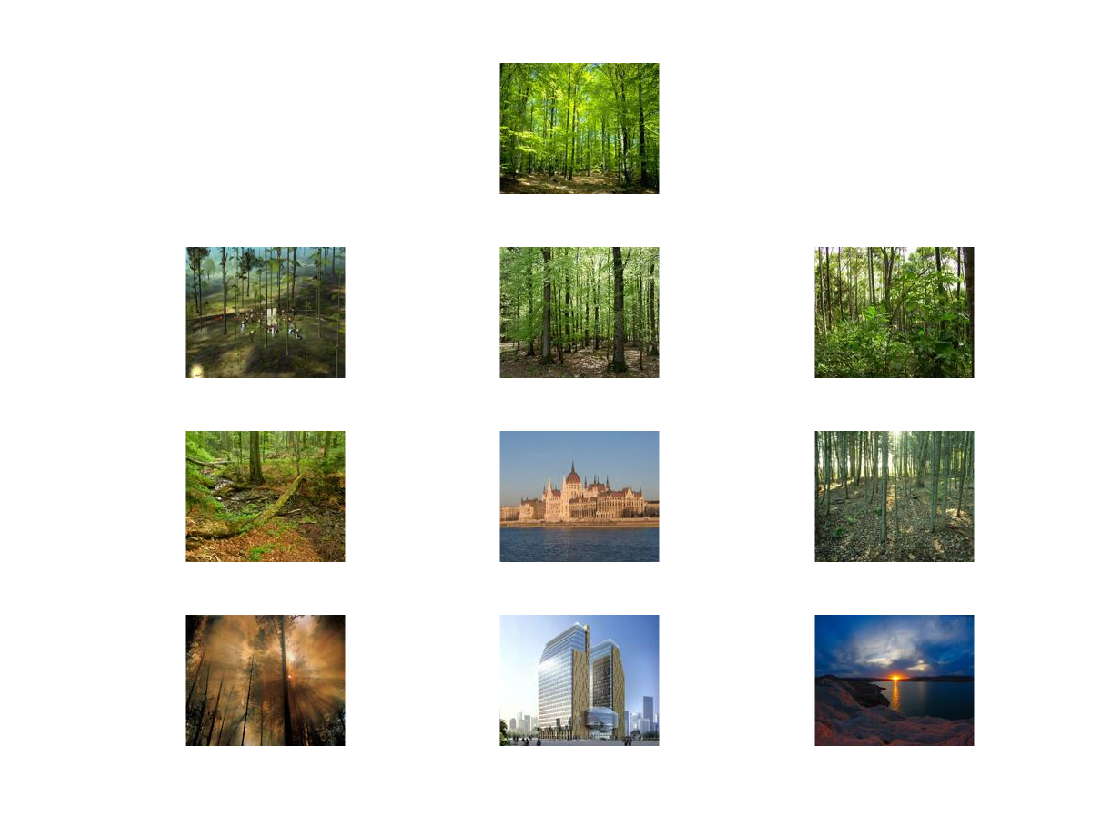
\includegraphics[width=0.45\textwidth]{img/f9knn_111110}}
\subfigure[\texttt{buildings\_5}]{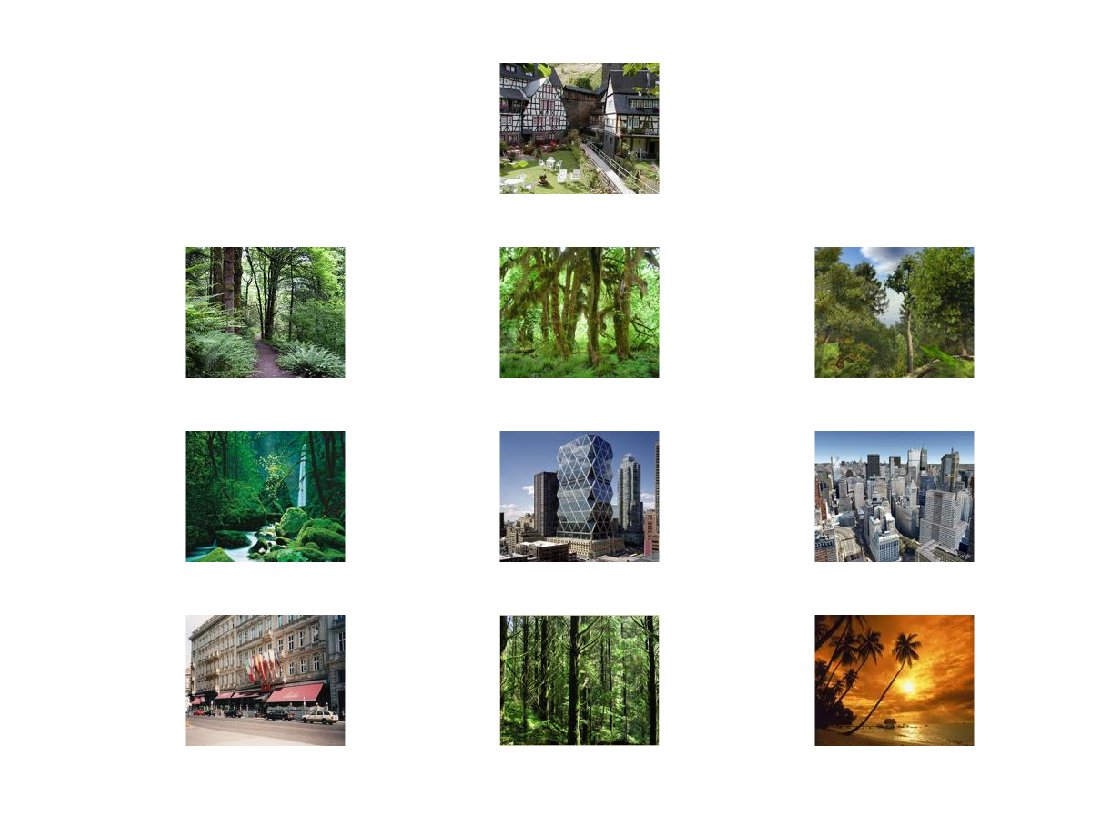
\includegraphics[width=0.45\textwidth]{img/b5knn_111110}}
\caption{Example KNN results using mean, standard deviation, minimum, maximum and median}
\label{fig:111110}
\end{figure}

The next step of experimenting involves adding color features to the feature space. The filters of the LM filter bank were all applied on gray scale images and ignore color differences. Thus, we add three new features for each image: the mean values for all color channels red (R), blue (B), and green (G). It turns out that these 3 features are well suited to separate the classes, as can be seen in figure \ref{fig:mrgb}.  


\begin{figure}[!hbt]
\centering
\subfigure[R channel vs G channel]{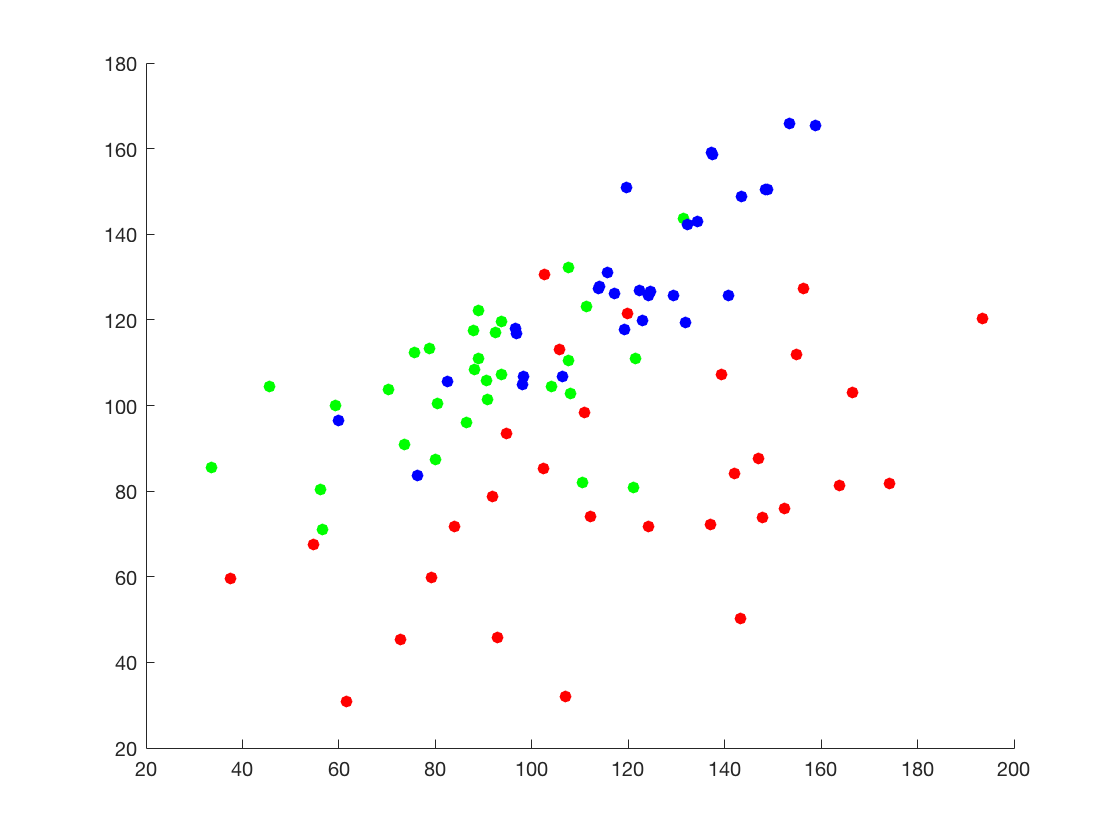
\includegraphics[width=0.33\textwidth]{img/mr_mg}}
\subfigure[R channel vs B channel]{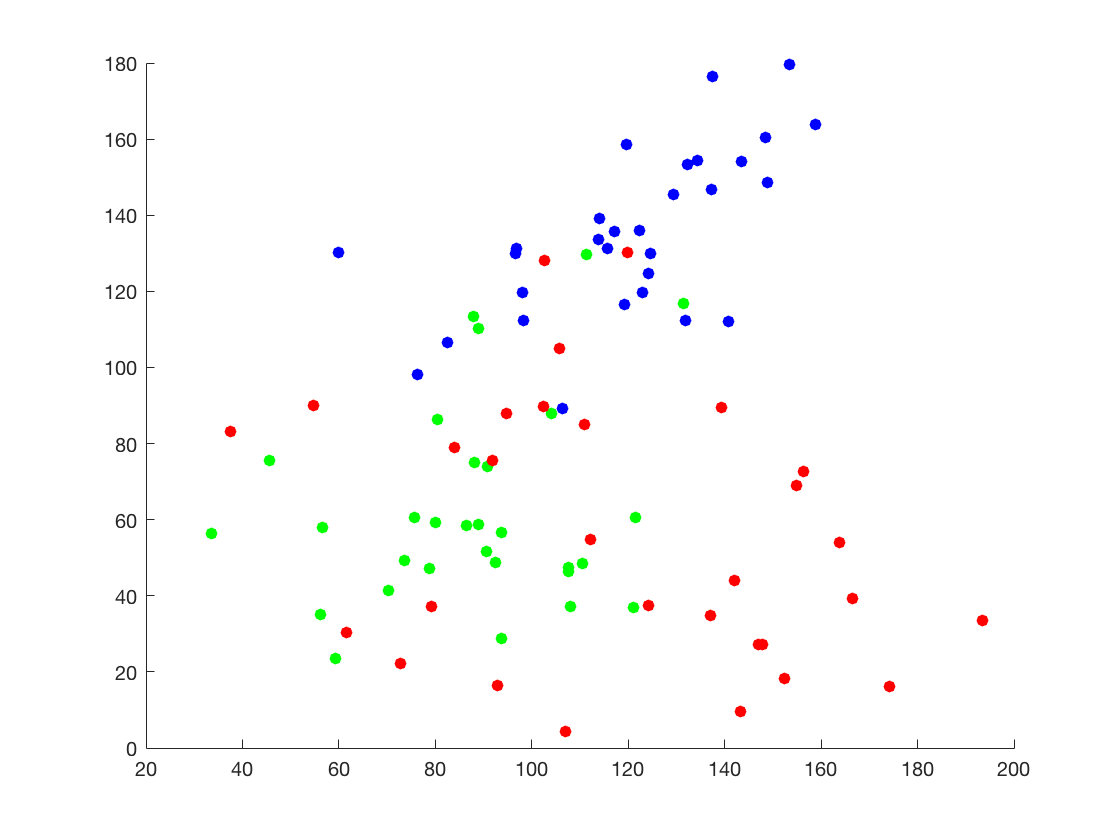
\includegraphics[width=0.33\textwidth]{img/mr_mb}}
\subfigure[B channel vs G channel]{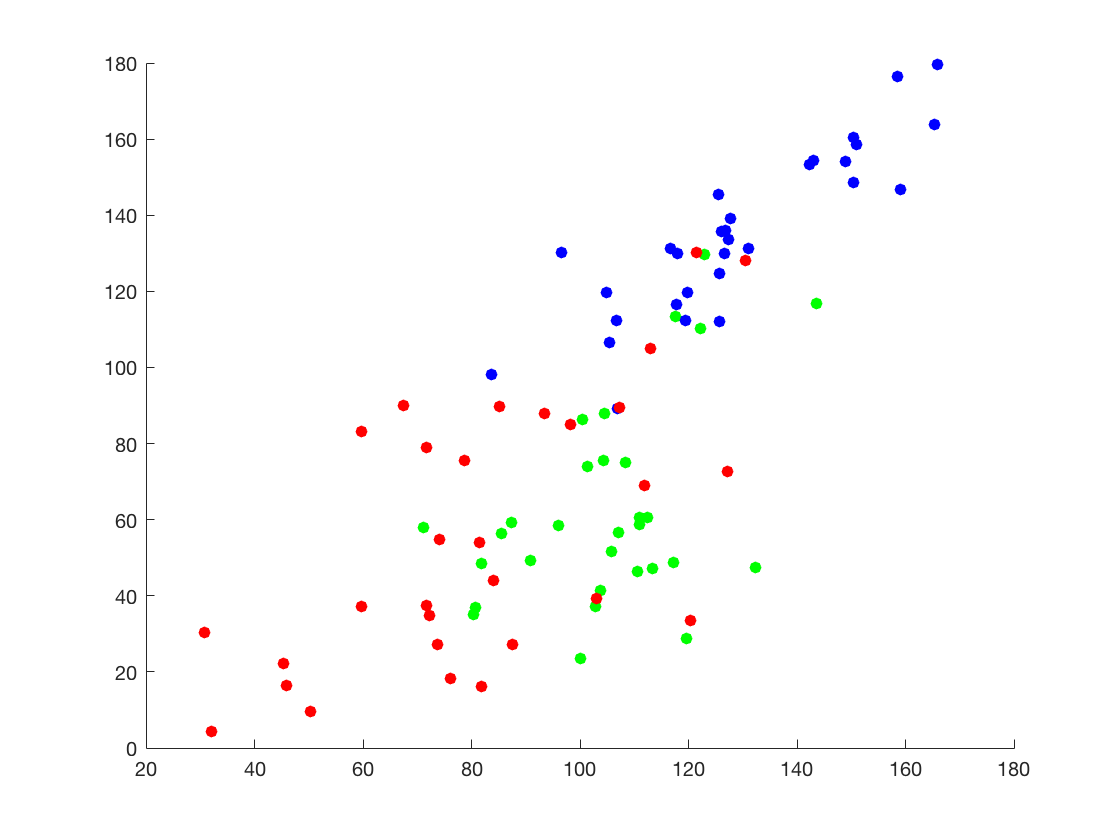
\includegraphics[width=0.33\textwidth]{img/mb_mg}}
\caption{Separability of RGB features}
\label{fig:mrgb}
\end{figure}

Figure \ref{fig:000001} shows the results of the KNN algorithm when only using the three mean color values as features. The results are very good for the forest example, but much less so for the buildings example that now gets confused with a variety of forests, buildings and sunsets.
\begin{figure}[!hbt]
\centering
\subfigure[\texttt{forest\_9}]{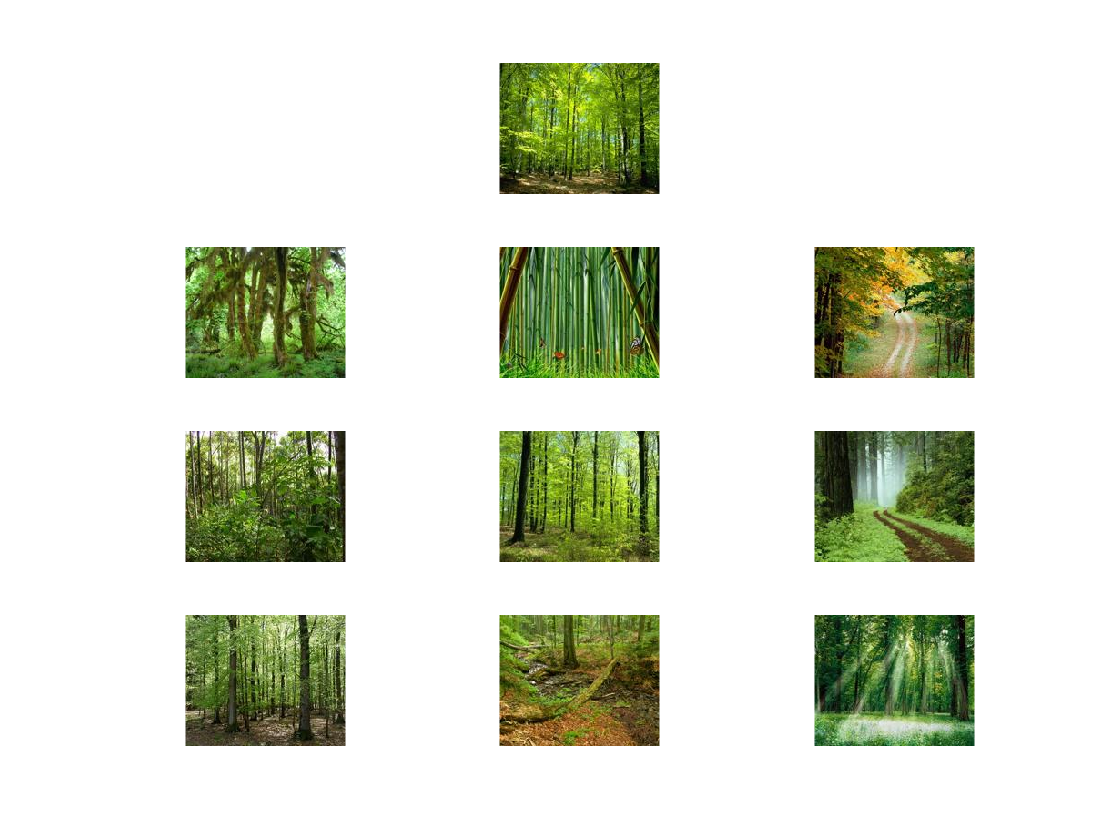
\includegraphics[width=0.45\textwidth]{img/f9knn_000001}}
\subfigure[\texttt{buildings\_5}]{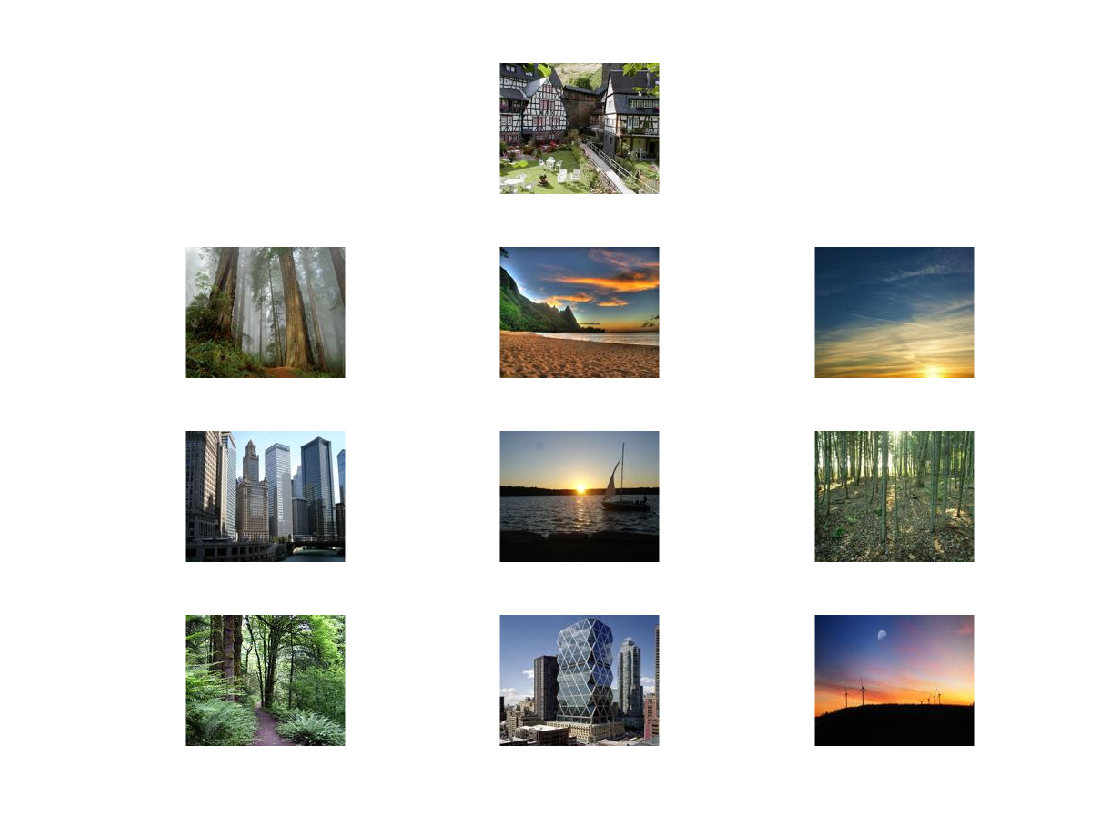
\includegraphics[width=0.45\textwidth]{img/b5knn_000001}}
\caption{Example KNN results for RGB based features}
\label{fig:000001}
\end{figure}

When adding the means of responses back to the filter set, the results for the forest decrease, but the retrieved images for \texttt{building\_5} are significantly better, as can be seen in figure \ref{fig:100001}.

\begin{figure}[!hbt]
\centering
\subfigure[\texttt{forest\_9}]{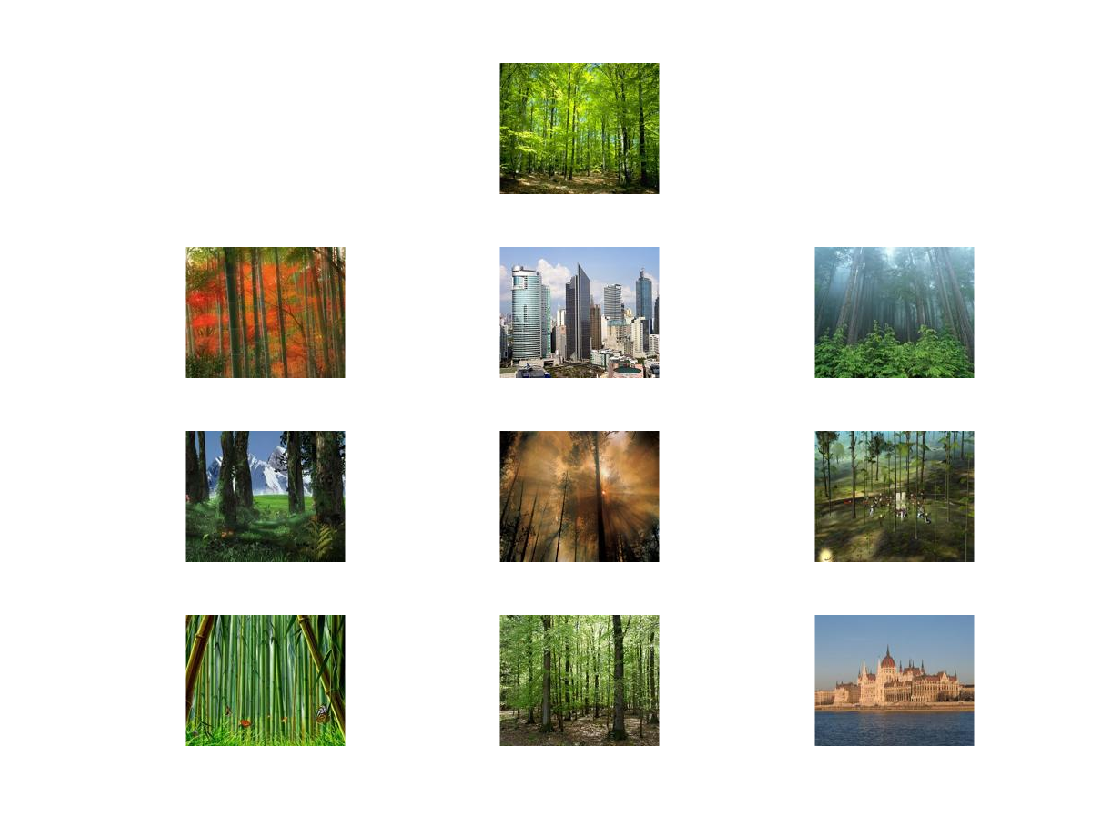
\includegraphics[width=0.45\textwidth]{img/f9knn_100001}}
\subfigure[\texttt{buildings\_5}]{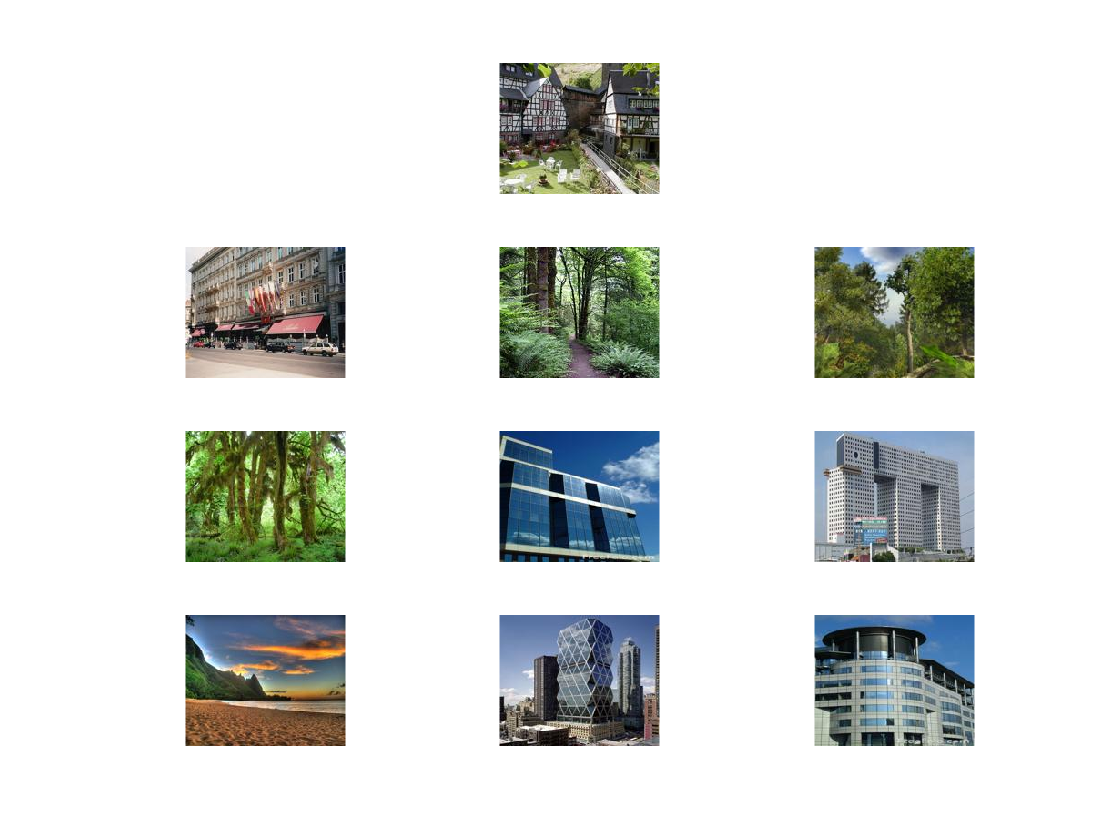
\includegraphics[width=0.45\textwidth]{img/b5knn_100001}}
\caption{Example KNN results for mean and RGB based features}
\label{fig:100001}
\end{figure}

The best results for the two examined cases are obtained when using a combination of standard deviations of responses to the texture filters and the color features, as depicted in figure \ref{fig:010001}

\begin{figure}[!hbt]
\centering
\subfigure[\texttt{forest\_9}]{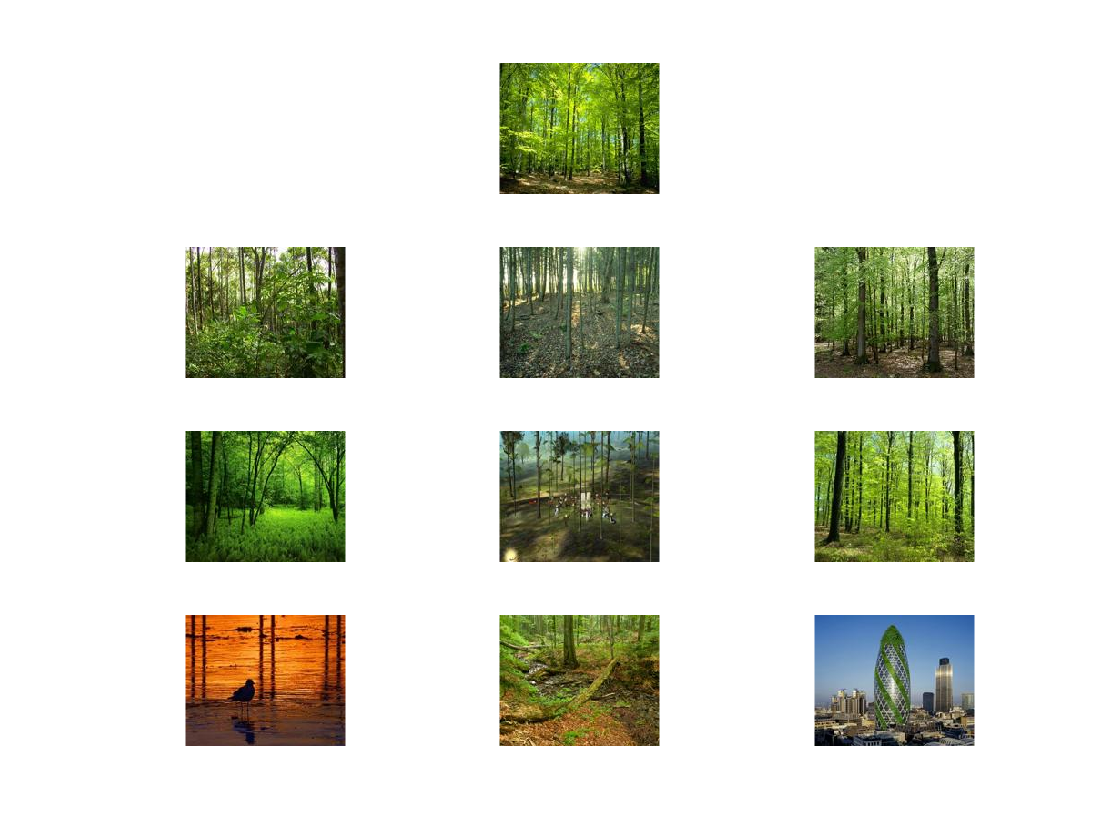
\includegraphics[width=0.45\textwidth]{img/f9knn_010001}}
\subfigure[\texttt{buildings\_5}]{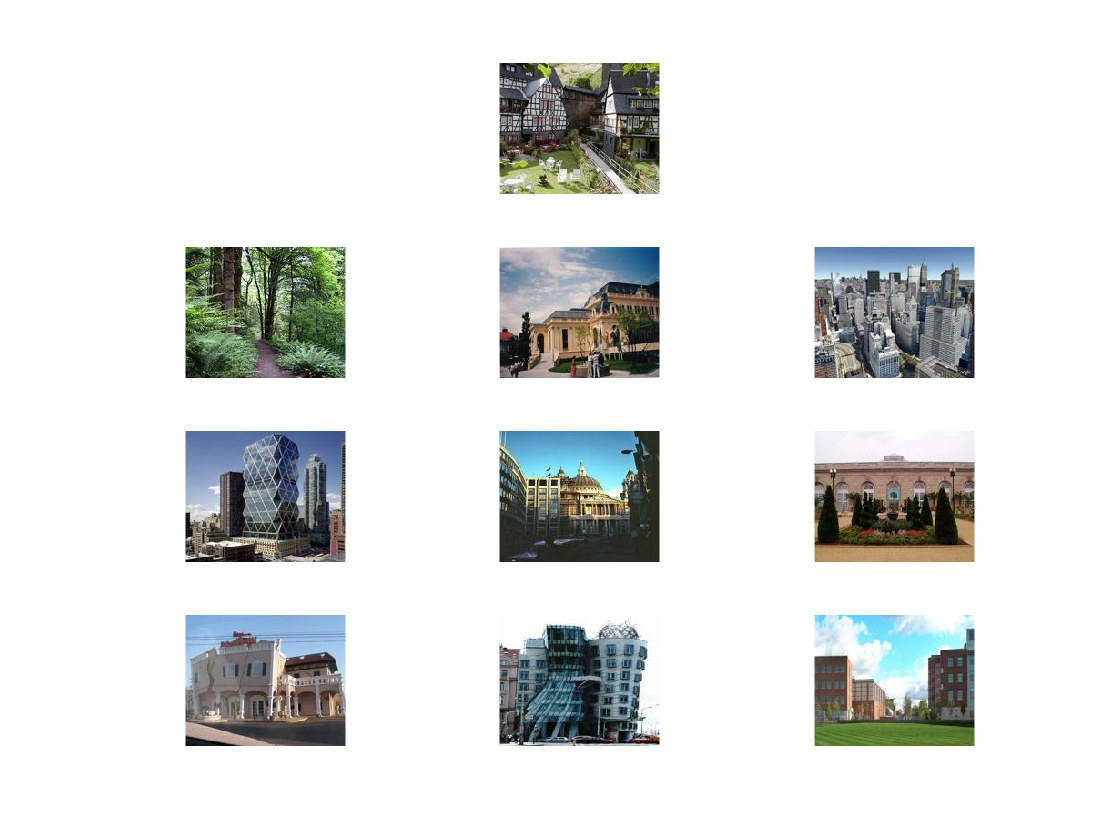
\includegraphics[width=0.45\textwidth]{img/b5knn_010001}}
\caption{Example KNN results for standard deviation and RGB based features}
\label{fig:010001}
\end{figure}

In addition to looking at individual examples of knn-search results using different sets of features, we tried to quantify the quality of a feature set by measuring, how often the 9 images retrieved for each image belong to the same class as the queried image, and how often they come from other classes. Based on that we can calculate the accuracy for different choices of features. It is important to note that this metric does not actually provide the accuracy of retrieving similar images, but only the accuracy of retrieving images of the same class. One can argue, however, that these metrics would yield at least similar results. In the following table we summarize the results of this experiment:
\vspace{1em}

\begin{table}[!hbt]
\centering
	\begin{tabular}{|c|c|c|c|c|c|c|}
  \hline
  \textbf{mean} & \textbf{stdev} & \textbf{min} & \textbf{max} & \textbf{median} & \textbf{RGB} & \textbf{accuracy} \\
  \hline
  \textbf{yes} & no & no & no & no & no & 0.42 \\
  \hline
  no & \textbf{yes} & no & no & no & no & 0.63 \\
  \hline
  no & no & \textbf{yes} & no & no & no & 0.58 \\
  \hline
  no & no & no & \textbf{yes} & no & no & 0.53 \\
  \hline
  no & no & no & no & \textbf{yes} & no & 0.40 \\
  \hline
  no & no & no & no & no & \textbf{yes} & 0.76 \\
  \hline
  \textbf{yes} & no & no & no & no & \textbf{yes} & 0.53 \\
  \hline
  no & \textbf{yes} & no & no & no & \textbf{yes} & 0.71 \\
  \hline
  no & no & \textbf{yes} & no & no & \textbf{yes} & 0.59 \\
  \hline
  no & no & no & \textbf{yes} & no & \textbf{yes} & 0.69 \\
  \hline
  no & no & no & no & \textbf{yes} & \textbf{yes} & 0.50 \\
  \hline
  \textbf{yes} & \textbf{yes} & \textbf{yes} & \textbf{yes} & \textbf{yes} & no & 0.46 \\
  \hline
  \textbf{yes} & \textbf{yes} & \textbf{yes} & \textbf{yes} & \textbf{yes} & \textbf{yes} & 0.51 \\
  \hline
  \end{tabular}
  \caption{Comparing classification accuracy for different feature sets}
  \label{tab:1}
\end{table}

As we can see in table \ref{tab:1}, the accuracy of classification varies quite a lot based on which features we select to be included in the knn-search. If we only choose one aggregation method for the filter responses, standard deviation achieves the highest accuracy with 63\% of retrieved similar images actually belonging to the same class as the queried image. One surprising observation is, that simply using the mean value of each image's color channels RGB yields by far the highest accuracy of 76\%. Adding any kind of aggregated texture feature decreases the results for this metric. It is likely that a learned weighting of color and texture features would result in even higher accuracy, but this was sadly beyond the scope of this report. If a single texture feature had to be selected, the obvious choice for the given three classes would be the standard deviation - it achieved the highest results both with RGB features and without them.
